\chapter{Resultados}
\label{chapter:Resultados}

Neste capítulo, serão apresentados os principais resultados obtidos referentes ao desenvolvimento do SocialFramework. Esses resultados foram obtidos através da análise da cobertura do código fonte, da complexidade dos algoritmos utilizados e da qualidade do código.

\section{Testes Unitários}

Durante o desenvolvimento do SocialFramework foi elaborada uma suíte de testes para tentar garantir que cada ponto do código funcione da devida maneira. Desse modo, o desenvolvedor pode inserir novos códigos, módulos ou alterar um código existente, com mais tranquilidade e sabendo que o restante do código irá funcionar adequadamente. Caso algum resultado esperado seja diferente do obtido, a suíte de testes irá apontar a falha.

Para a realização dos testes, foi utilizada a \textit{gem} do Rspec\footnote{\url{http://rspec.info/}}. Essa \textit{gem} é amplamente utilizada pela comunidade do Rails. E para a visualização do relatório de testes, foi utilizado o Code Climate\footnote{\url{https://codeclimate.com/}}, que é uma ferramenta \textit{online} que realiza uma análise estática do código fonte. Atualmente, são suportadas as linguagens: Ruby, Python, JavaScript e PHP.

No início do desenvolvimento, foi estabelecida uma meta de que se deveria testar no mínimo 90\% do código fonte. Essa meta foi cumprida, obtendo-se 98,8\% de cobertura do código. Porém essa métrica não corresponde à realidade, pois o arquivo ``engine.rb'', que teve sua cobertura de 47.83\%, é um arquivo de configuração do \textit{framework} e não deveria ser testado, e os arquivos  ``elements\_factory.rb'', ``elements\_factory\_default.rb'' e ``graph\_elements.rb'' tiveram a cobertura, respectivamente, de 60\%, 80\% e 84\%, diminuindo a cobertura real do código fonte. Entretanto, esses arquivos possuem classes ``abstratas'' e deveriam ser desconsiderados. Porém, em Ruby, não existe o conceito de classe abstrata. Olsen em seu livro \cite{Olsen:2007}, apresenta uma abordagem de se obter esse conceito. Um exemplo dessa abordagem pode ser observado, conforme consta no \ref{listing:classe_abstrata}:

 \begin{lstlisting}[
    label=listing:classe_abstrata,
    caption=Classe abstrata,
    numbers=left,
    language=Ruby,
    basicstyle=\footnotesize\sffamily,
    keywordstyle=\color{red},
    stringstyle=\color{blue},
]
# Define abstract methods to Vertex
class Edge
  attr_accessor :origin, :destiny, :labels
  
  # Constructor to Edge
  # ====== Params:
  # +origin+:: +Vertex+ relationship origin
  # +destiny+:: +Vertex+ relationship destiny
  # Returns NotImplementedError
  def initialize origin, destiny
    raise 'Must implement method in subclass'
  end
end
\end{lstlisting}

A seguir, são apresentados, na Figura \ref{Cobertura_teste} cada arquivo e sua respectiva cobertura.

\begin{figure}[!h]
	\centering
	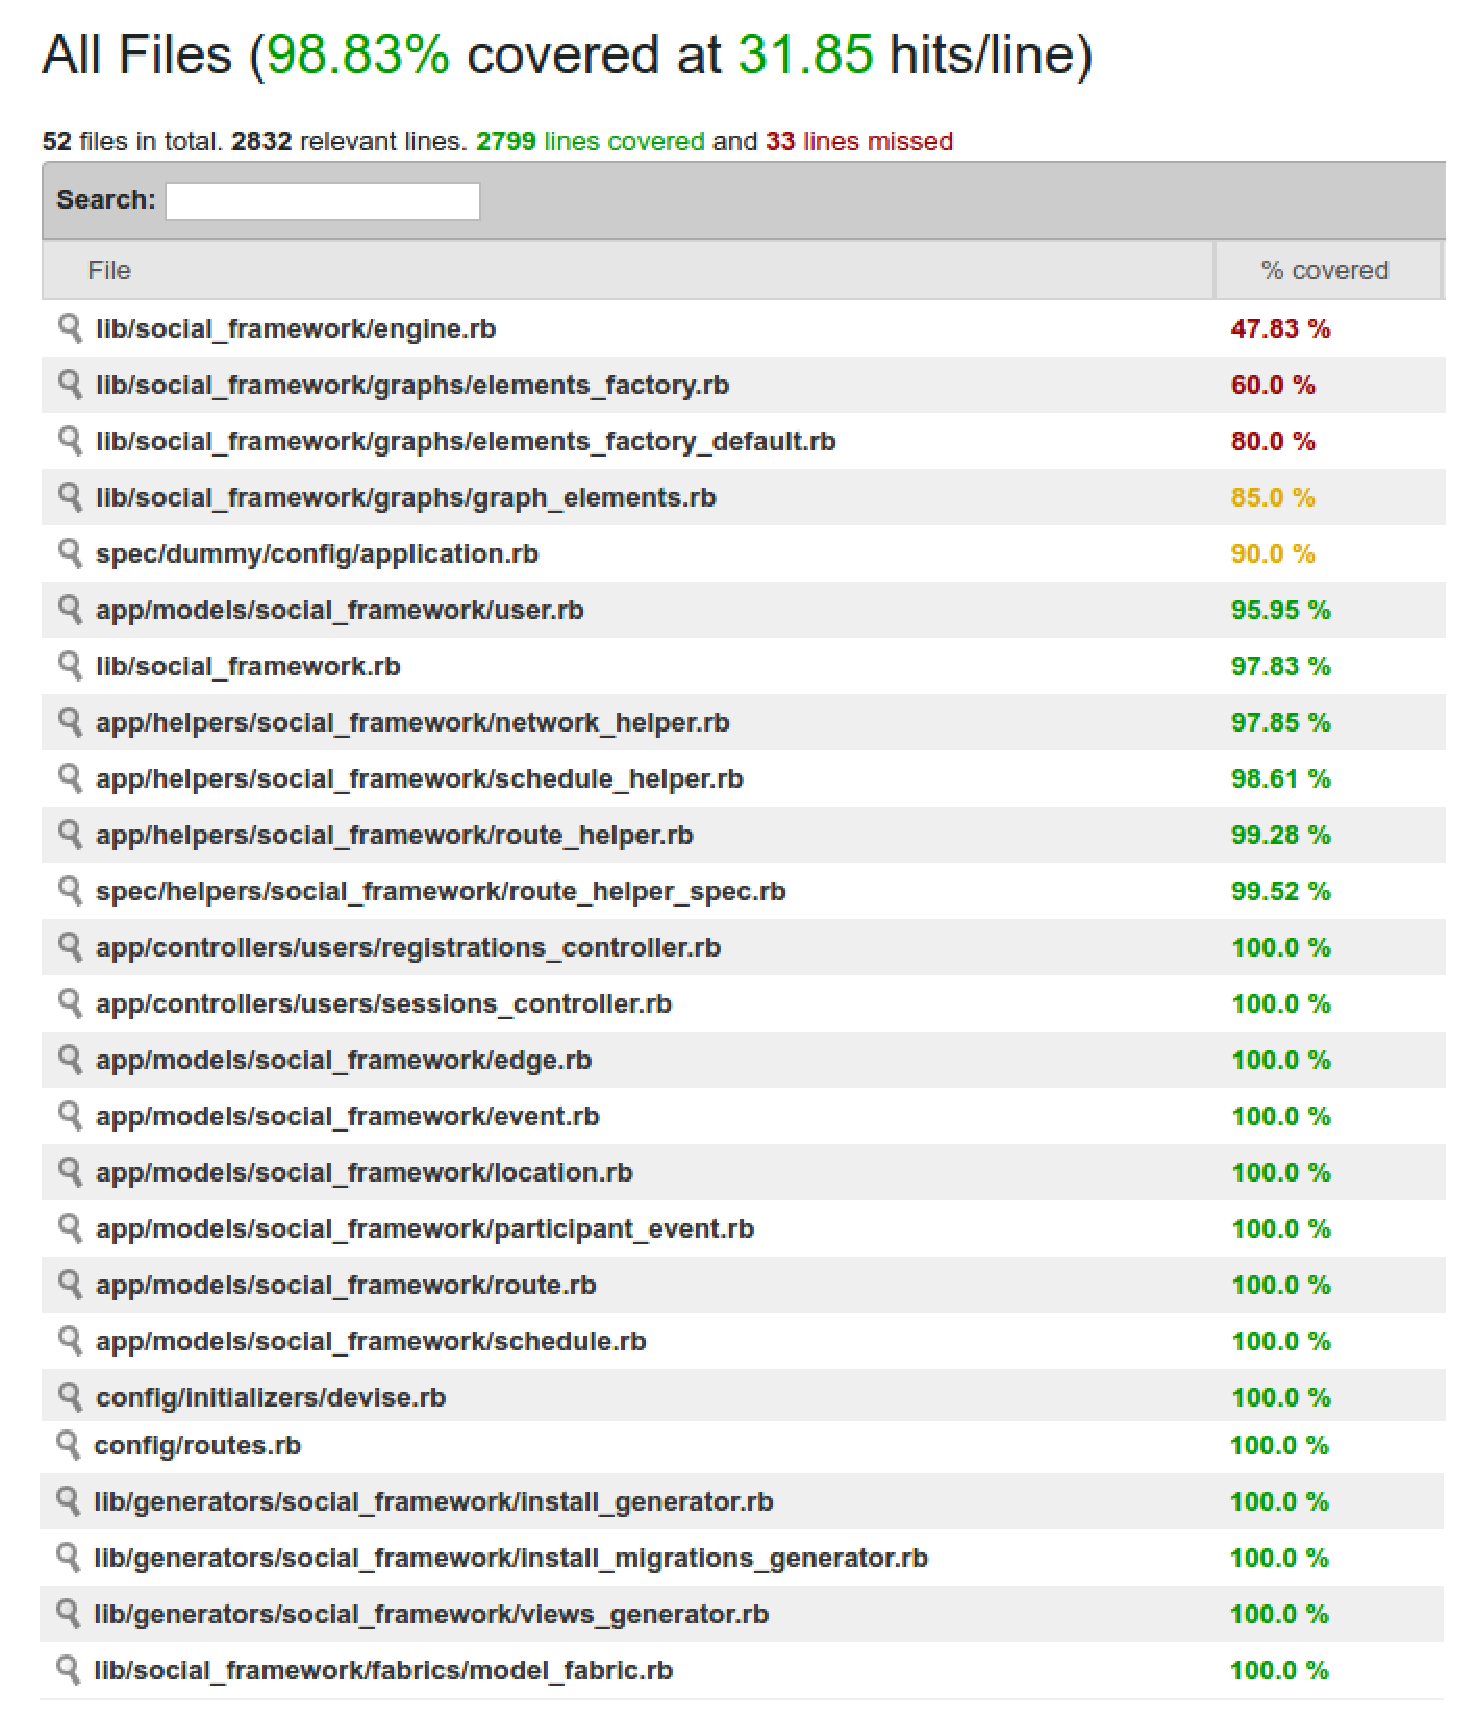
\includegraphics[scale=0.60]{figuras/resultados/cobertura.eps}
	\caption[Cobertura de teste]{Cobertura de teste}
	\label{Cobertura_teste}
\end{figure}

\section{Relatório de Desempenho}

Após a verificação do correto fluxo que o \textit{framework} executa, foram realizados testes de desempenho do mesmo, analisando o tempo de execução e o consumo de memória dos principais algoritmos desenvolvidos. Não foram realizados esses teste no módulo de rotas, pois os seus métodos fazem somente requisições de rotas à API do Google Maps e comparações sobre essas rotas.

Para se obter cada valor, foram feitas cinco medições, e foi realizada a média aritmética dos valores.

\subsection{Módulo de Usuário}

Para o módulo de usuário foram, realizados testes com 10 mil usuários, onde a quantidade de relacionamentos que os usuários possuíam em cada teste variou entre 100 relacionamentos, 200 relacionamentos, 300 relacionamentos, 400 relacionamentos e 500 relacionamentos. Para todos esses casos, cada usuário estava presente em 10 eventos.

\subsubsection{Tempo de Execução}

Para o método ``build'', que é responsável por construir o grafo a partir de um usuário raiz, foi especificado que o grafo deveria ser construído com três níveis de profundidade. Foi obtido o gráfico da Figura \ref{build_tempo} como resultado.

\begin{figure}[!h]
	\centering
	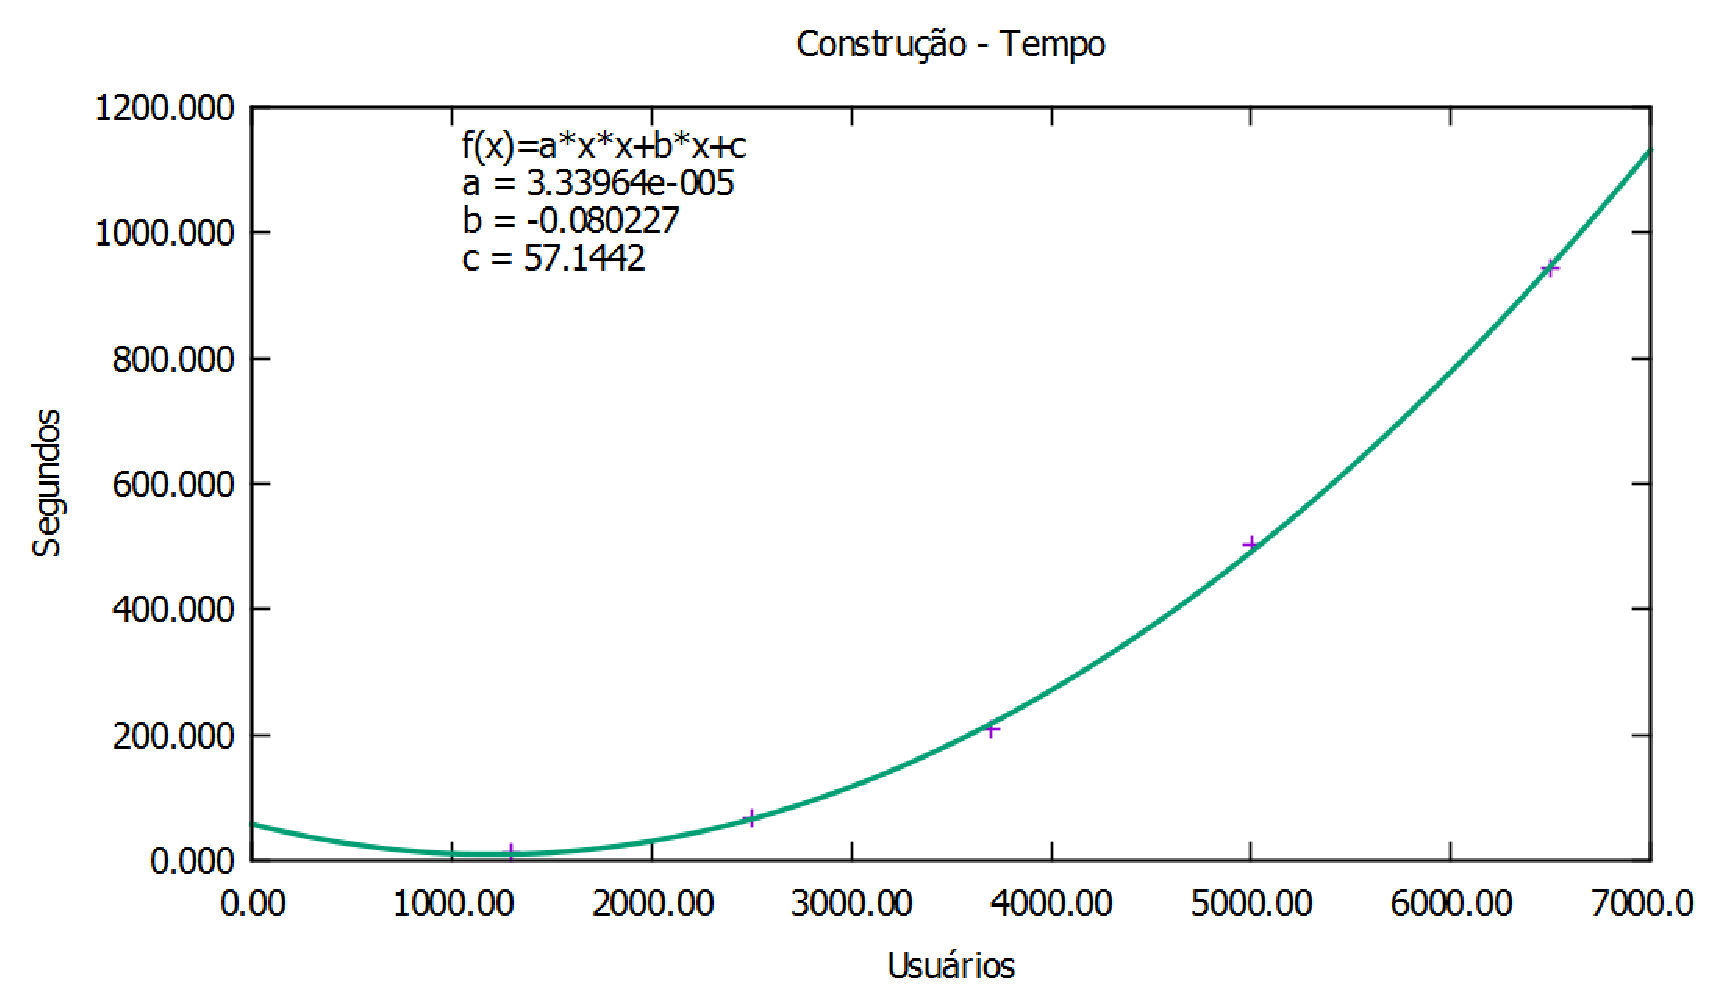
\includegraphics[scale=0.55]{figuras/resultados/graficos/construcao_tempo.eps}
	\caption[Construção]{Construção}
	\label{build_tempo}
\end{figure}

Para o método ``search'', que é responsável por fazer pesquisas no grafo, foram feitos dois tipos de pesquisas. A pesquisa padrão é uma pesquisa na qual serão encontrados os vértices até o segundo nível do grafo. O resultado desta pesquisa pode ser observado na Figura \ref{pesquisa_padrao}.

\begin{figure}[!h]
	\centering
	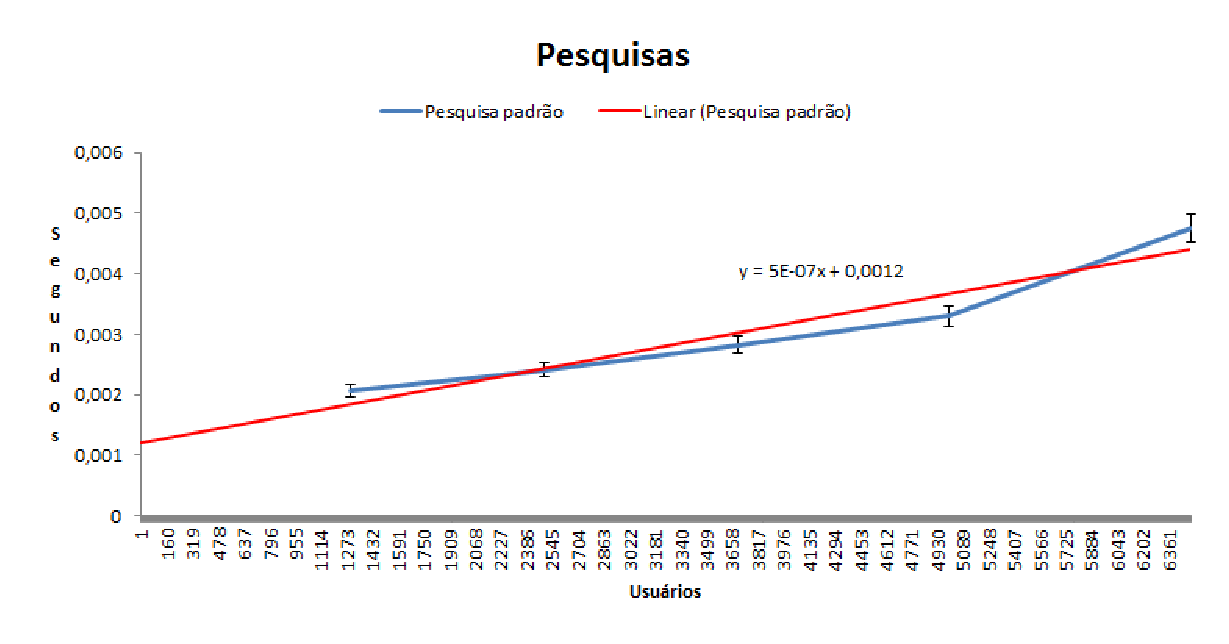
\includegraphics[scale=0.55]{figuras/resultados/graficos/pesquisa_padrao.eps}
	\caption[Pesquisa Padrão]{Pesquisa padrão}
	\label{pesquisa_padrao}
\end{figure}

A pesquisa no terceiro nível é uma pesquisa que irá percorrer até o último nível do grafo. Pode-se visualizar o resultado dessa pesquisa na Figura \ref{pesquisa_3}.

\newpage

\begin{figure}[!h]
	\centering
	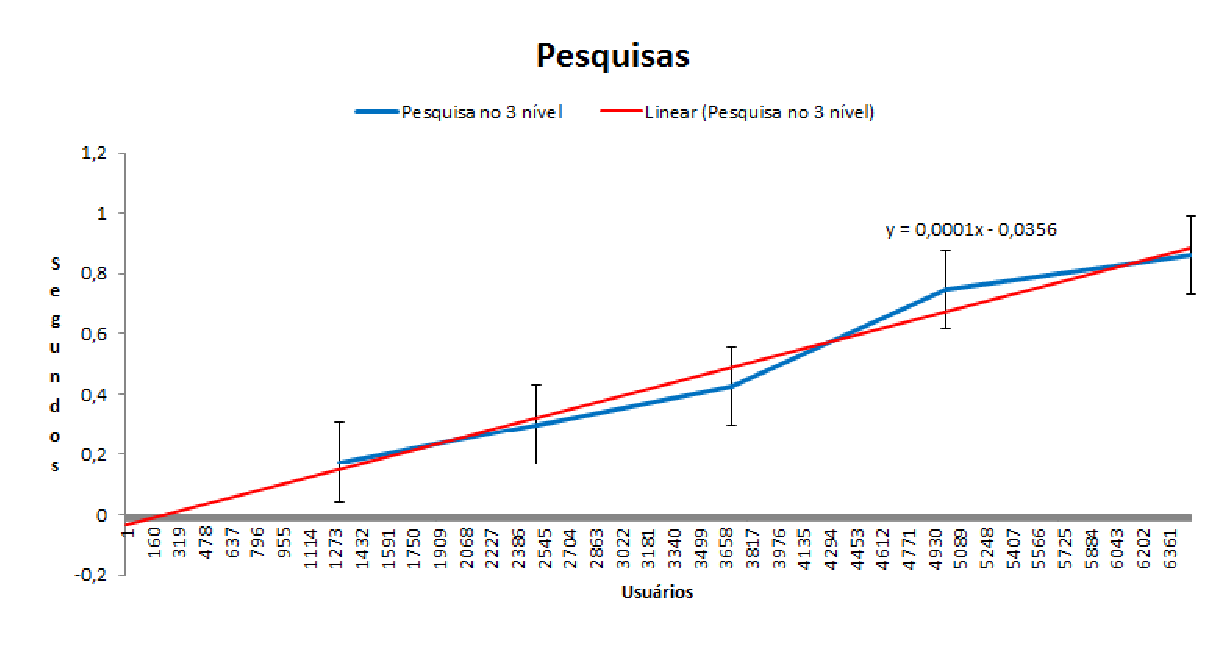
\includegraphics[scale=0.55]{figuras/resultados/graficos/pesquisa_3_nivel.eps}
	\caption[Pesquisa no terceiro nível]{Pesquisa no terceiro nível}
	\label{pesquisa_3}
\end{figure}

Para o método ``suggest\_relationships'', foi utilizado o parâmetro padrão para a quantidade de relacionamento para realizar a sugestão, que é cinco. Os tempos de execução para esse método podem ser visualizados na Figura \ref{suggest}.

\begin{figure}[!h]
	\centering
	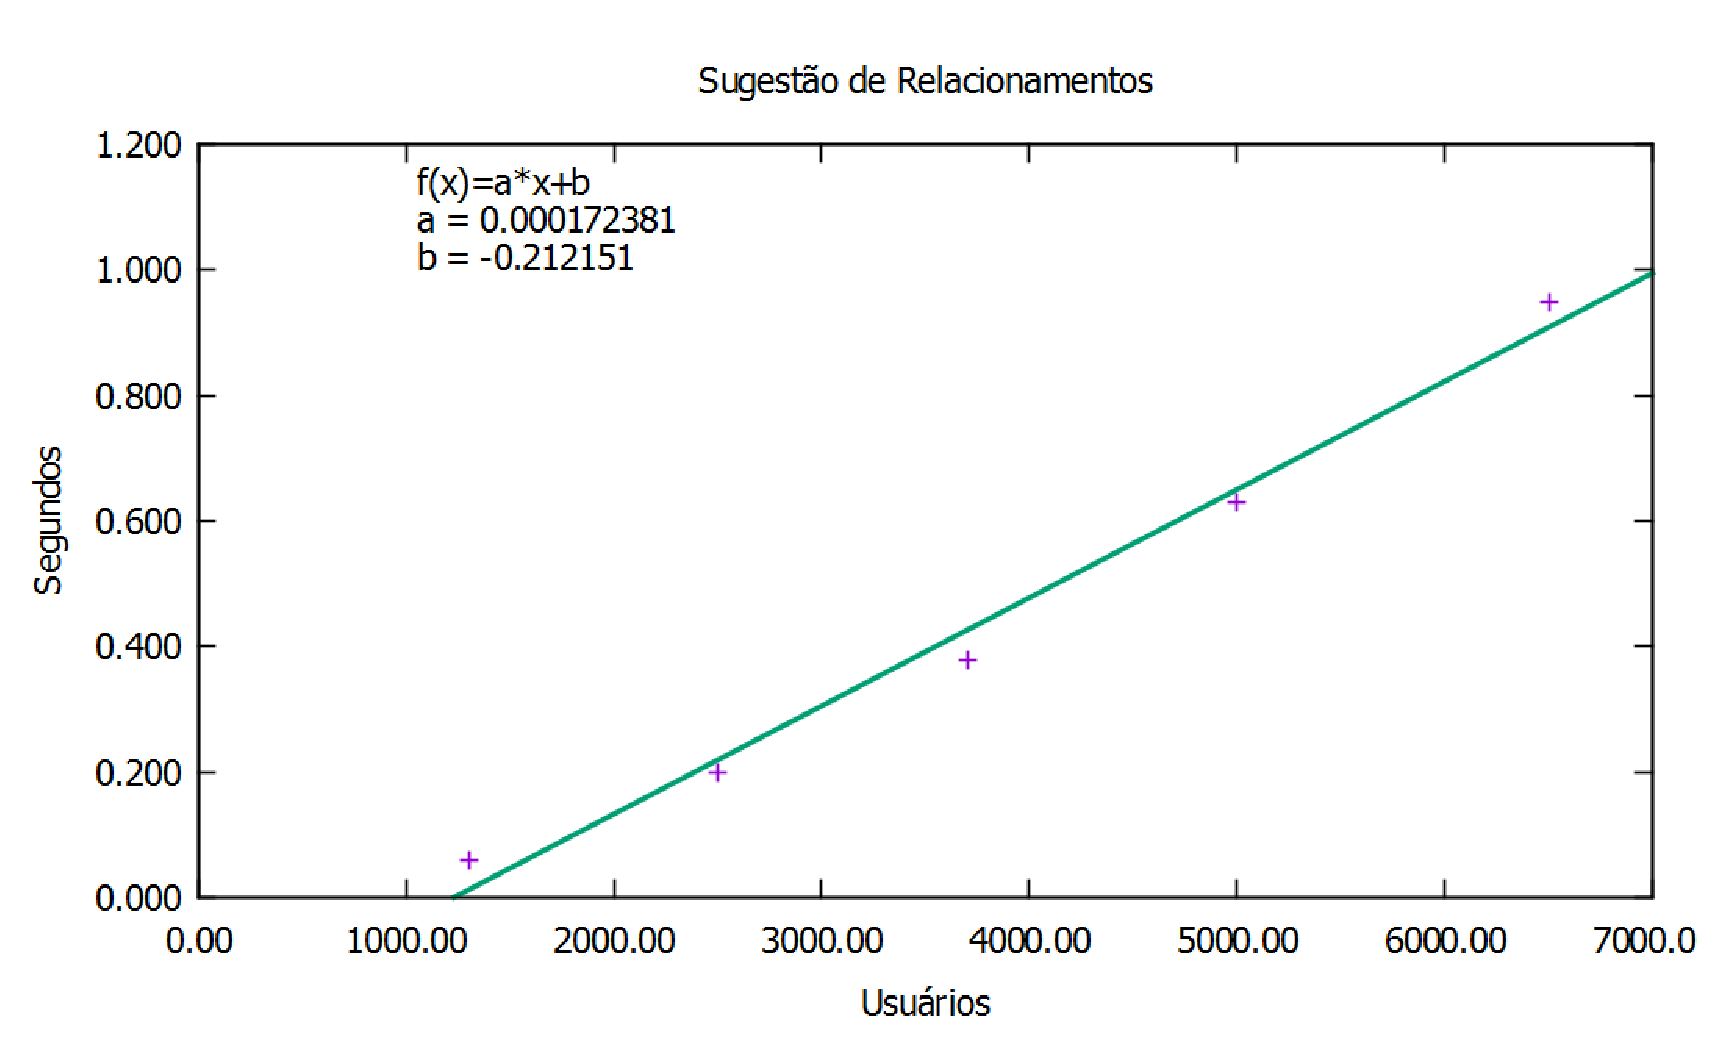
\includegraphics[scale=0.55]{figuras/resultados/graficos/sugestao_relacionamentos.eps}
	\caption[Sugestão de relacionamentos]{Sugestão de relacionamentos}
	\label{suggest}
\end{figure}

\subsubsection{Consumo de Memória}

O consumo de memória que o método ``build'' utilizou pode ser visualizado na Figura \ref{build_memoria}.

\begin{figure}[!h]
	\centering
	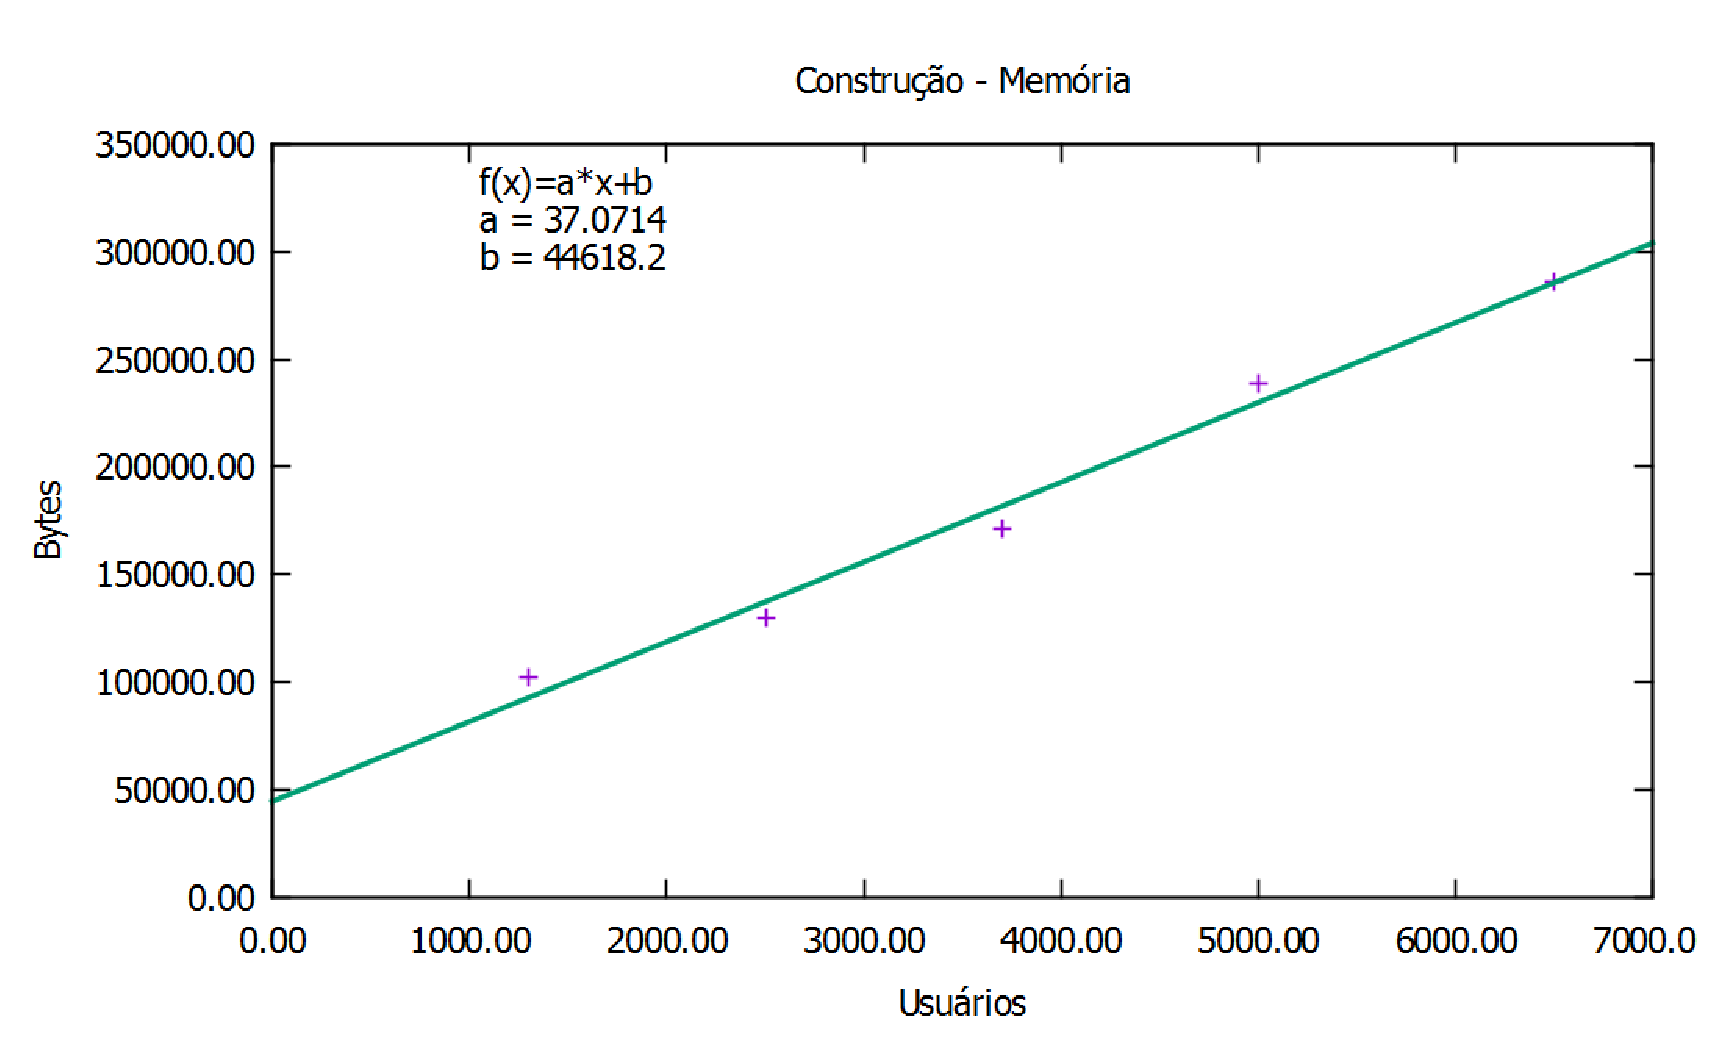
\includegraphics[scale=0.55]{figuras/resultados/graficos/construcao_memoria.eps}
	\caption[Consumo de memória do método build]{Consumo de memória do método \textit{build}}
	\label{build_memoria}
\end{figure}

Os métodos ``search'' e ``suggest\_relationships'', que tiveram seus tempos de execução apresentados na seção anterior não tiveram o seu consumo de memória medido, pois esses apenas utilizam a instância do grafo gerado pelo método ``build''.

\subsection{Módulo de Agenda}

No módulo de agenda, o método que teve o seu desempenho medido foi o ``verify\_availabilities'', o qual verifica o melhor horário para um evento levando em consideração um conjunto de usuários. Para tal, fui utilizado o \textit{slot} com o tamanho de 1 hora e considerou-se que os eventos poderiam ser marcados no horário de 08:00 às 12:00.

Para esse método, devem ser consideradas duas variáveis que podem influenciar o seu desempenho, que são o número de usuários e o intervalo de tempo. Portanto, foram feitas duas baterias de testes. Cada bateria de teste tinha uma dessas variáveis fixa. Já a outra era alterada.

\subsubsection{Intervalo de Tempo Fixo}

Com o intervalo de tempo fixo, foram feitos testes com o número de usuários variando a partir dos valores: 10, 50, 100, 300 e 500.

A seguir, é apresentado, na Figura \ref{31dias_tempo}, o tempo de execução do método ``verify\_availabilities'' com o intervalo de tempo de 31 dias.

\begin{figure}[!h]
	\centering
	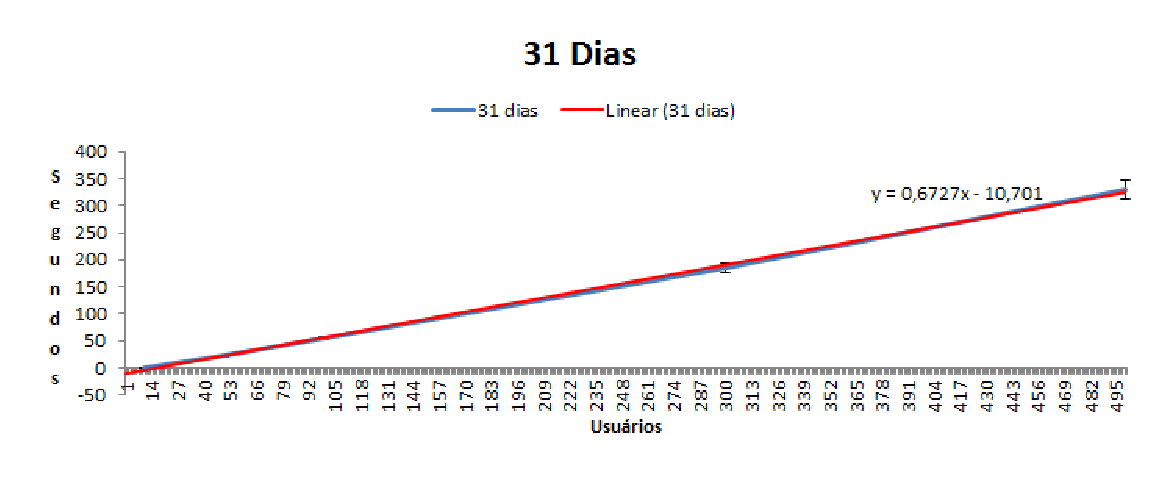
\includegraphics[scale=0.55]{figuras/resultados/graficos/31_dias_tempo.eps}
	\caption[Tempo de execução com disponibilidade de 31 dias]{Tempo de execução com disponibilidade de 31 dias}
	\label{31dias_tempo}
\end{figure}

Na Figura \ref{31dias_memoria}, pode-se visualizar a quantidade de memória consumida com um intervalo de tempo de 31 dias.

\begin{figure}[!h]
	\centering
	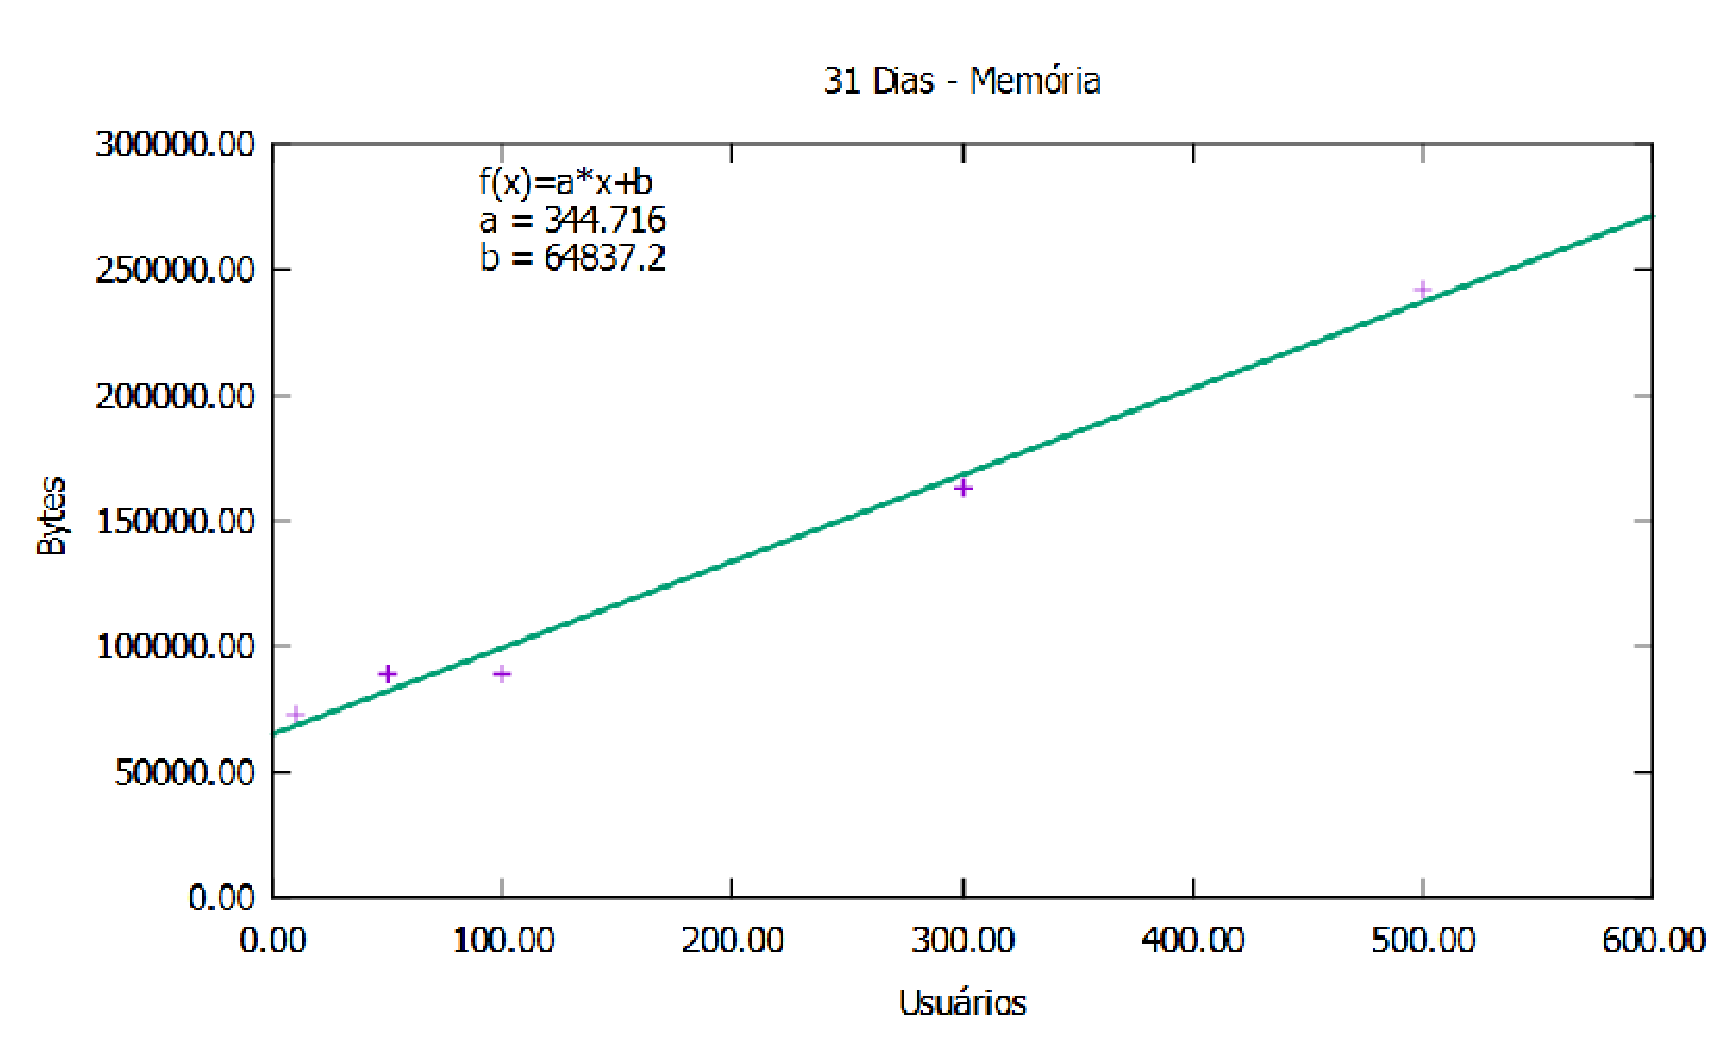
\includegraphics[scale=0.55]{figuras/resultados/graficos/31_dias_memoria.eps}
	\caption[Consumo de memória com disponibilidade de 31 dias]{Consumo de memória com disponibilidade de 31 dias}
	\label{31dias_memoria}
\end{figure}

\subsubsection{Número de Usuários Fixo}

Com o número de usuários fixo, foram realizados testes com o intervalo de tempo variando entre 7, 15, 31, 45 e 60 dias.

É possível observar na Figura \ref{500users_tempo} o tempo de execução quando o número de usuários é fixo em 500 e o intervalo de tempo é variável.

\begin{figure}[!h]
	\centering
	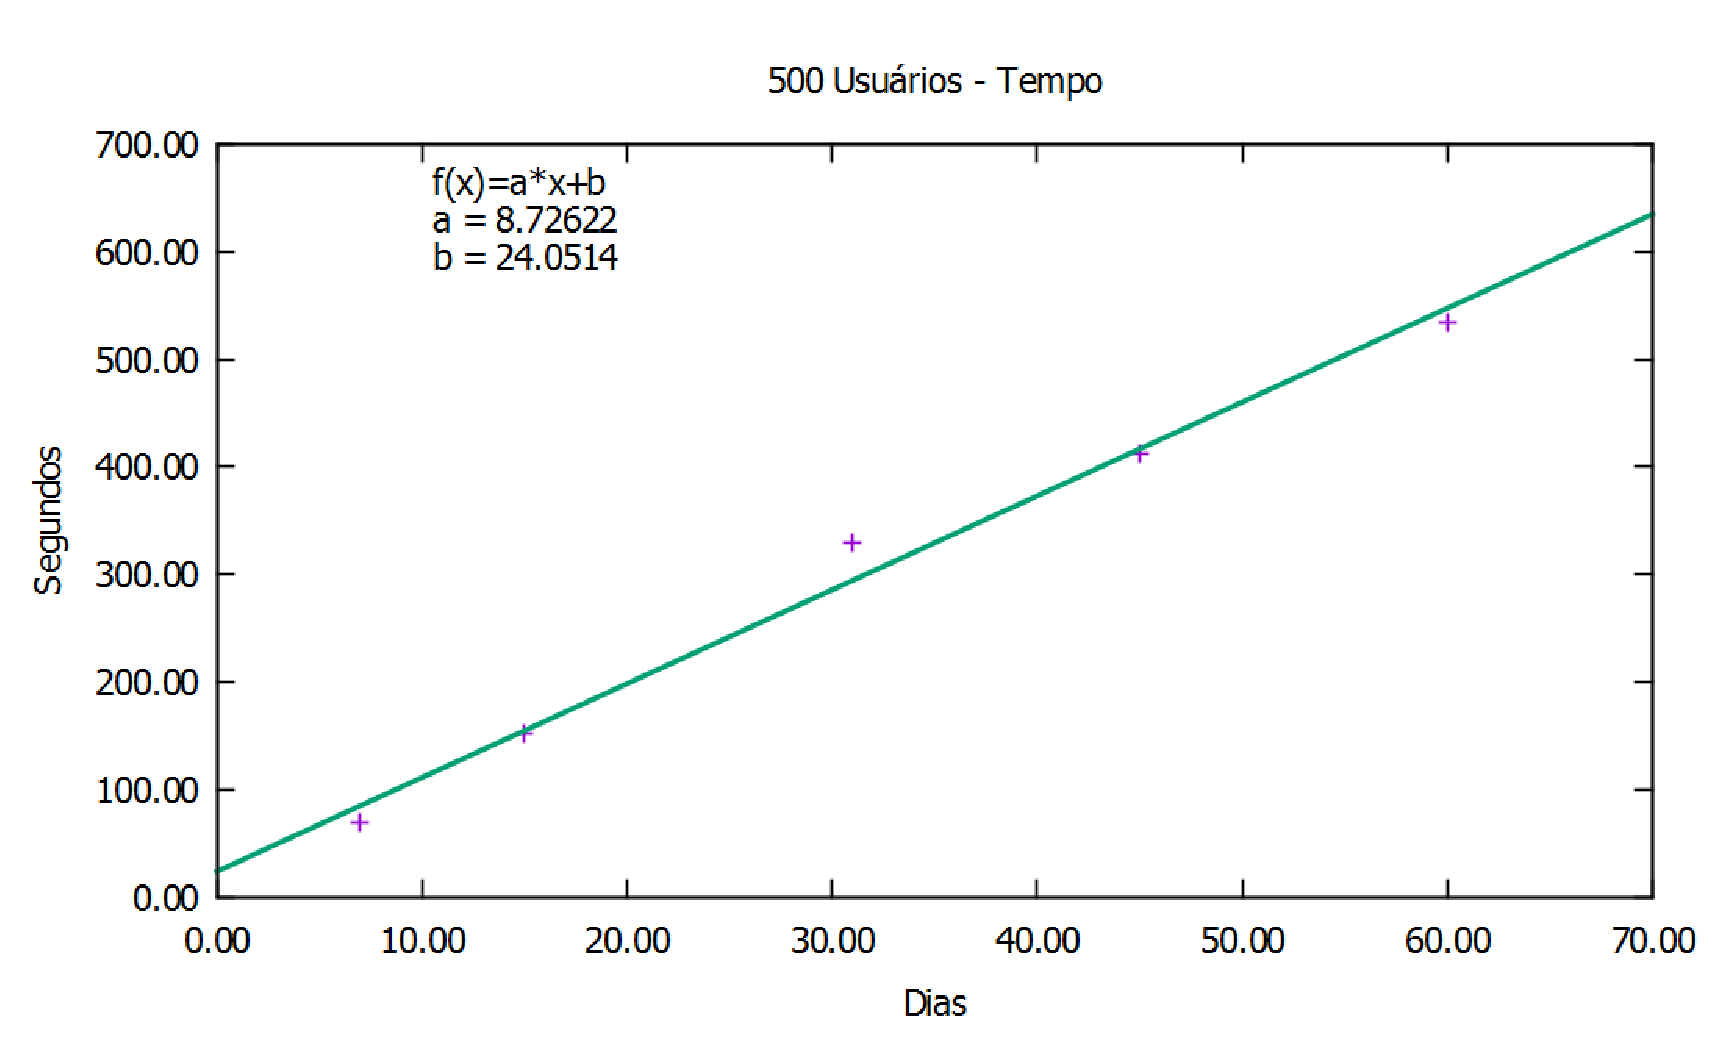
\includegraphics[scale=0.55]{figuras/resultados/graficos/500_users_tempo.eps}
	\caption[Tempo de execução para 500 usuários]{Tempo de execução para 500 usuários}
	\label{500users_tempo}
\end{figure}

A quantidade de memória consumida com 500 usuários fixos, pode ser observada na Figura \ref{500users_memoria}.

\newpage

\begin{figure}[!h]
	\centering
	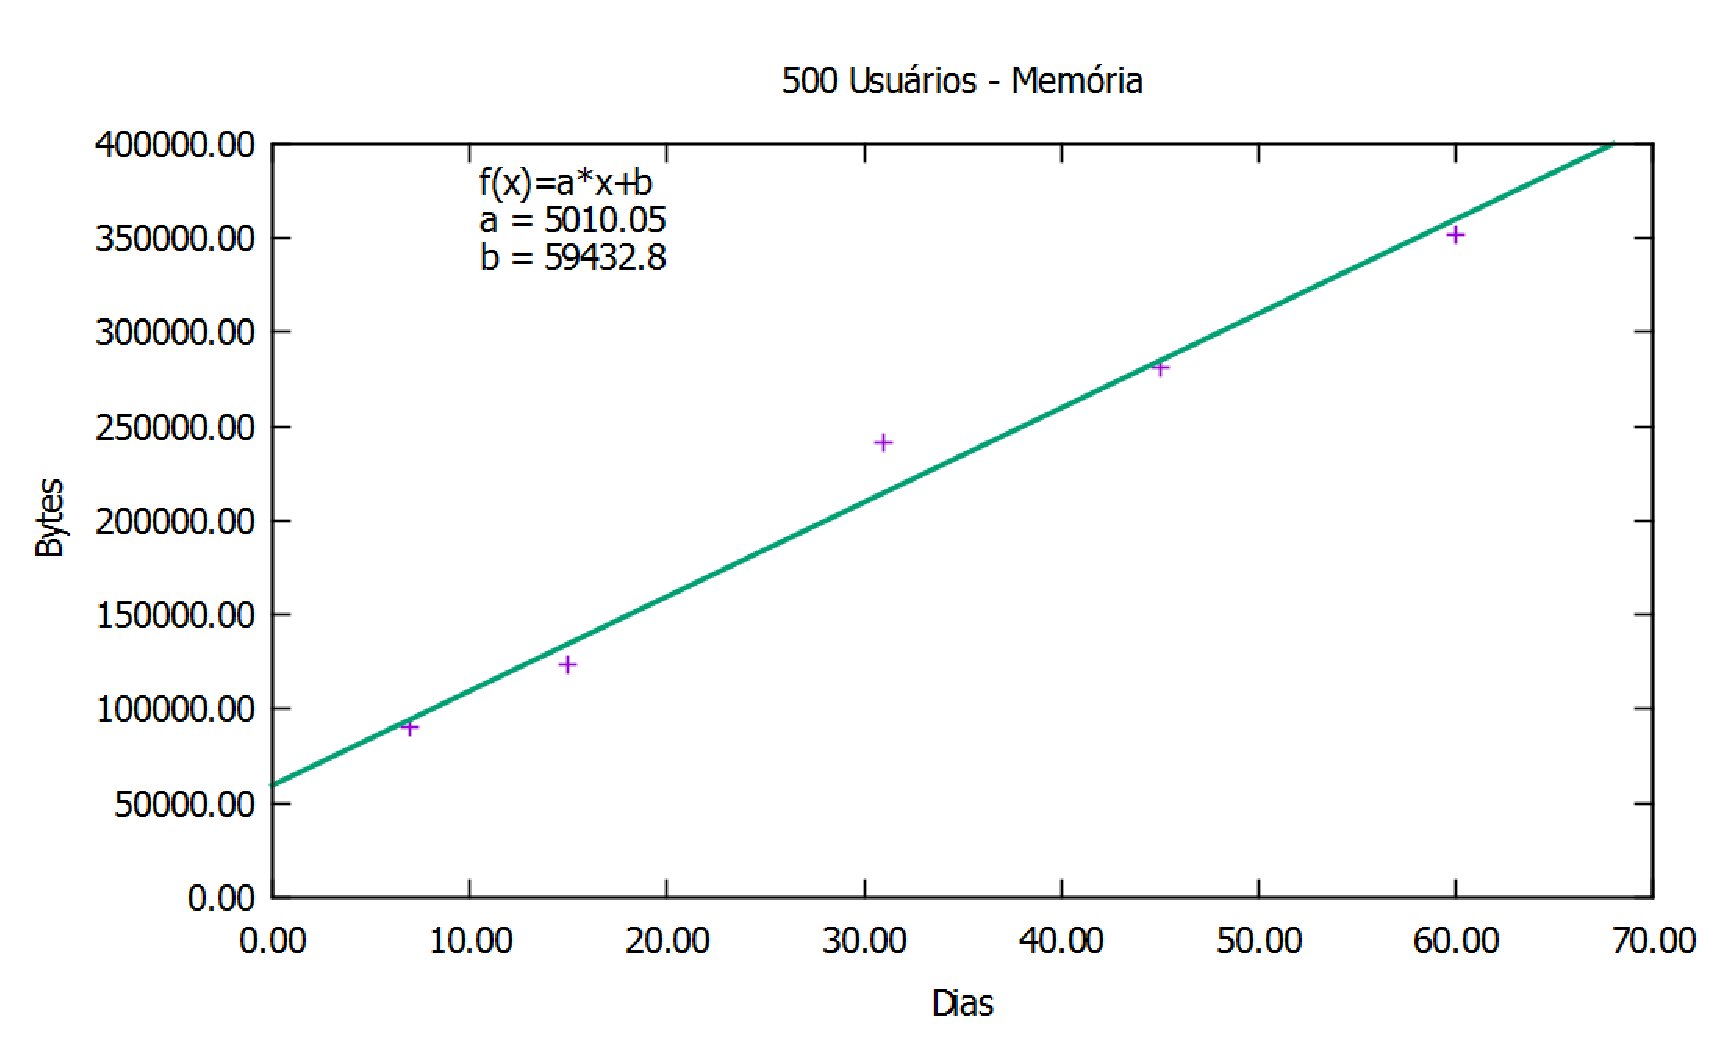
\includegraphics[scale=0.55]{figuras/resultados/graficos/500_users_memoria.eps}
	\caption[Consumo de memória para 500 usuários]{Consumo de memória para 500 usuários}
	\label{500users_memoria}
\end{figure}

\subsection{Complexidade}

A partir dos gráficos apresentados anteriormente e da pesquisa realizada e documentada na seção \nameref{sec:complexidade_algoritmos}, pode-se avaliar a complexidade dos algoritmos utilizados.

O tempo para a construção do grafo têm sua função aproximada a uma equação de \textit{x*log(x)}. Portanto, pode-se concluir que esse método possuem uma complexidade em seu tempo de O(n*log(n)). Já o tempo nos algoritmos de pesquisa, de sugestão de relacionamentos, e de verificar a disponibilidade de agendas tiveram o seu tempo de execução aproximados a uma reta. Portanto, esses algoritmos possui uma complexidade de tempo de execução de O(n).

O consumo de memória de todos os algoritmos que foram medidos tiveram os seus gráficos aproximados a uma reta. Desse modo pode dizer que esses algoritmos possuem uma complexidade de consumo de memória de O(n).

\section{Qualidade do SocialFramework}

Essa seção procurará exibir os resultados quanto à qualidade do código fonte do \textit{framework}. A partir da análise de código fonte realizada pela ferramenta Code Climate, foi possível obter as métricas e realizar uma análise qualitativa dos resultados obtidos.

Medir e monitorar a qualidade do software é fundamental. Mesmo uma ótima suíte de testes pode produzir informações apenas sobre características externas, não refletindo qualidades como manutenibilidade, modularidade, flexibilidade e simplicidade \cite{Filho:2013}.

Filho, em \cite{Filho:2013}, afirma ainda que nem tudo é relevante para ser controlado. Portanto, não se deve procurar medir tudo, mas escolher bem as métricas para avaliar e controlar o projeto. Desse modo, as métricas que foram monitoradas durante o projeto foram:

\begin{enumerate}
	\item \textbf{Complexidade}: Essa métrica fornece uma análise da complexidade e do esforço gasto em um trecho de código. Para tanto, foram utilizadas as seguintes métricas:
	\begin{enumerate}
		\item \textbf{Complexidade ciclomática}: é calculada pela quantidade de caminhos que é possível percorrer no método. Dessa forma, sempre começa em 1, pois todo método tem pelo menos um caminho possível. Para cada estrutura condicional ou repetitiva(\textit{if}, \textit{unless}, \textit{elsif}, \textit{while}, \textit{until}, \textit{for}, \textit{when}, \textit{rescue}), é adicionado mais 1 para a complexidade;
		\item \textbf{Tamanho do código}: que é a quantidade de linhas que o código possui, desconsiderando comentários e espaços em branco;
		\item \textbf{Complexidade ABC}: o cálculo da complexidade é baseado em três pontos:
		\begin{enumerate}
			\item \textbf{Assignment}: qualquer atribuição explícita de um dado para uma variável, por exemplo: = *= /= \%= += <<= >>= \&= |= >= ++ —, entre outros;
		    \item \textbf{Branch}: quando um caminho fora do escopo do programa é feito, por exemplo, uma chamada de método de instância de um objeto, um operador \textit{new} instanciando uma classe, etc;
    		\item \textbf{Condition}: qualquer teste lógico/booleano, == != <= >= < > \textit{else case default try catch} ? e condicionais unários.
		\end{enumerate}
	\end{enumerate}
	\item \textbf{Duplicação de código}: analisa a similaridade de trechos de código na aplicação. Para cada nível de similaridade, é atribuído um peso diferente, indo de similar até idêntico, resultando no número que é a somatória de todos os arquivos. Espaços em branco, nomes de variáveis, métodos e classes são ignorados pela ferramenta;
	\item \textbf{Estilo}: verifica se o projeto utiliza o guia de estilo descrito pela comunidade Rails. Aponta onde estão as práticas não adequadas relacionadas, relacionadas a padrões e convenções, as quais não estão sendo respeitadas na aplicação, e
	\item \textbf{Segurança}: utiliza um \textit{fork} do Brakeman na versão 2.6.2 para identificar as vulnerabilidades do projeto Rails.
\end{enumerate}

\newpage

A partir dessas métricas, o Code Climate realiza o cálculo do GPA (\textit{grade point average}) que é uma espécie de média de todos os arquivos do projeto. O GPA possui um intervalo de 0 a 4 pontos, levando em consideração as notas dos arquivos, que varia de `A' a `F'. Desse modo, no início do projeto, foi estabelecido uma meta de 3 pontos. Essa meta foi atingida com êxito, obtendo-se 3.45 pontos, como pode ser observado na Figura \ref{GPA}.

\begin{figure}[!h]
	\centering
	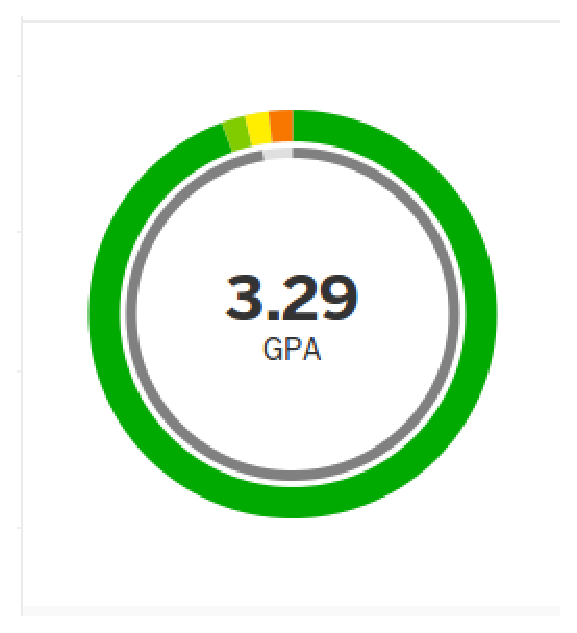
\includegraphics[scale=0.5]{figuras/resultados/gpa.eps}
	\caption[GPA]{GPA}
	\label{GPA}
\end{figure}

Esse valor do GPA foi obtido de acordo com a Tabela \ref{gpa_arquivos}, que ilustra a quantidade de arquivos com as notas de `A' até `F'.

\begin{table}[!h]
\centering
\caption{Nota de cada arquivo}
\label{gpa_arquivos}
\begin{tabular}{cccccc}
\toprule
\textbf{Nota A} & \textbf{Nota B} & \textbf{Nota C} & \textbf{Nota D} & \textbf{Nota E} & \textbf{Nota F} \\ \midrule
50 & 2 & 1 & 0 & 0 & 0							   \\ \bottomrule
\end{tabular}
\end{table}

\section{SocialBike}
\label{sec:SocialBike}

O SocialBike é a rede social desenvolvida para fazer uso do SocialFramework e, dessa forma, aplicá-lo em um uso real para comprovação de seus recursos. É uma rede voltada para ciclistas que auxilia os mesmos a, principalmente, marcarem eventos em comum para andar de bicicleta e/ou verificar rotas de outros usuários que coincidam com as suas. Nessa rede, foram desenvolvidas funcionalidades que perpassam pelos três módulos do SocialFramework, Usuários, Agenda e Rotas.

Para o módulo de usuários, foram desenvolvidas funcionalidades gerais de redes sociais, com cadastro de usuários, \textit{login}, relacionamentos e pesquisas. A seguir, são apresentadas uma sequência de imagens do SocialBike, com as telas dessas funcionalidades.

A Figura \ref{cadastrar_usuario} apresenta a tela de cadastro de usuários. Quando um usuário se cadastra na rede, esse é automaticamente logado na mesma.

\newpage
\begin{figure}[!h]
	\centering
	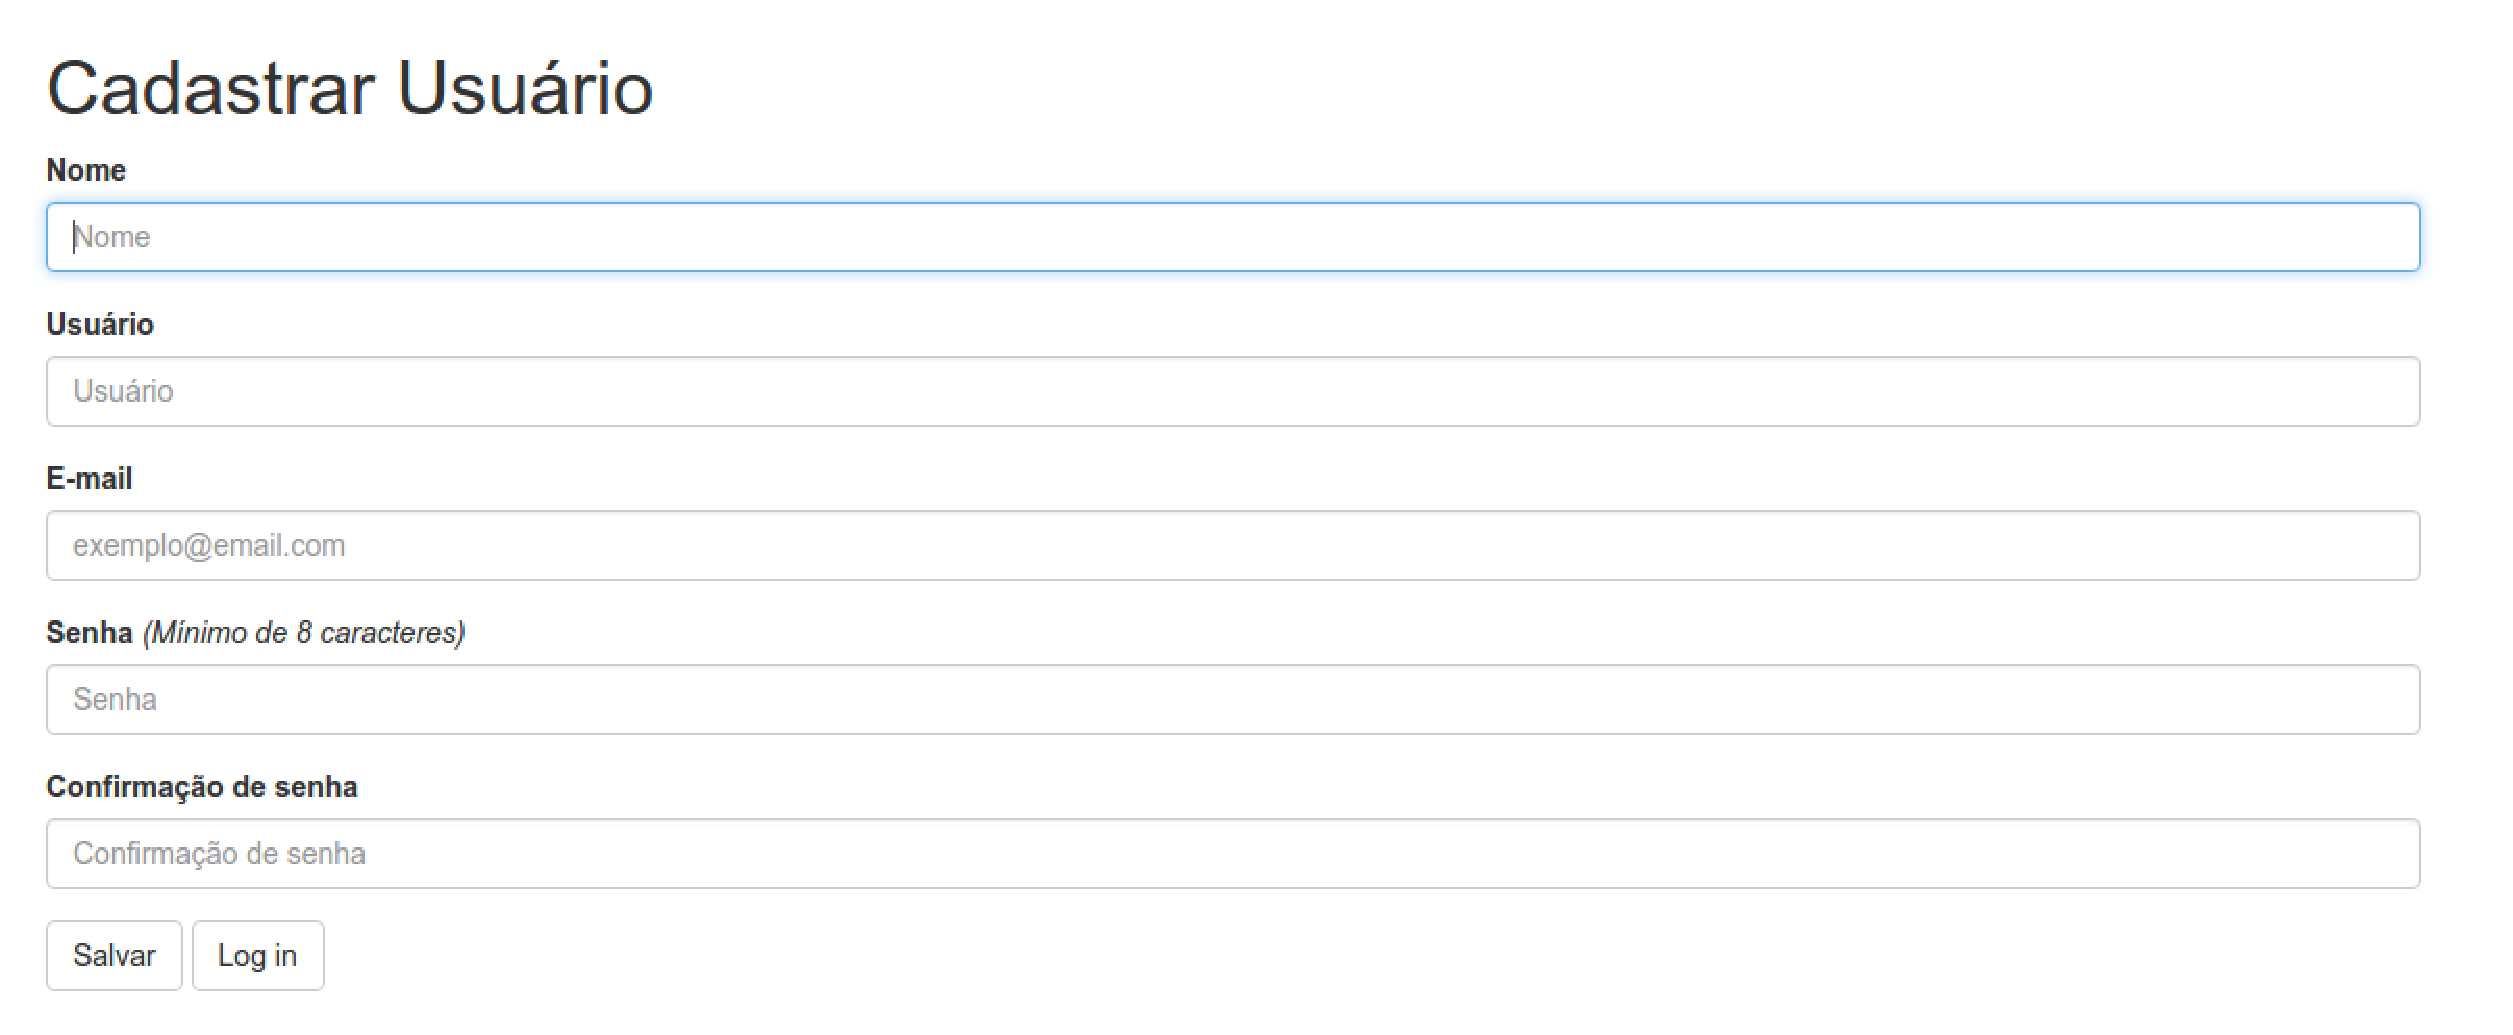
\includegraphics[scale=0.4]{figuras/resultados/cadastrar_usuario.eps}
	\caption[Tela de cadastro de usuários]{Tela de cadastro de usuários}
	\label{cadastrar_usuario}
\end{figure}

A Figura \ref{login} apresenta a tela para entrar na rede social.

\begin{figure}[!h]
	\centering
	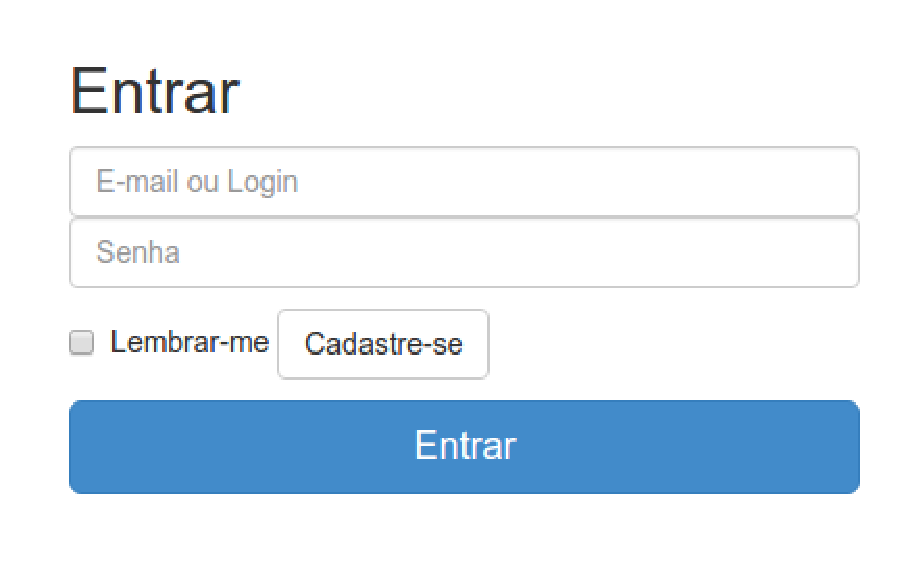
\includegraphics[scale=0.5]{figuras/resultados/login.eps}
	\caption[Tela de login]{Tela de \textit{login}}
	\label{login}
\end{figure}

A Figura \ref{home} mostra a tela principal da rede social, com as listas dos amigos e sugestões de amizades para o usuário logado, além de um campo para realização de pesquisas.

\newpage
\begin{figure}[!h]
	\centering
	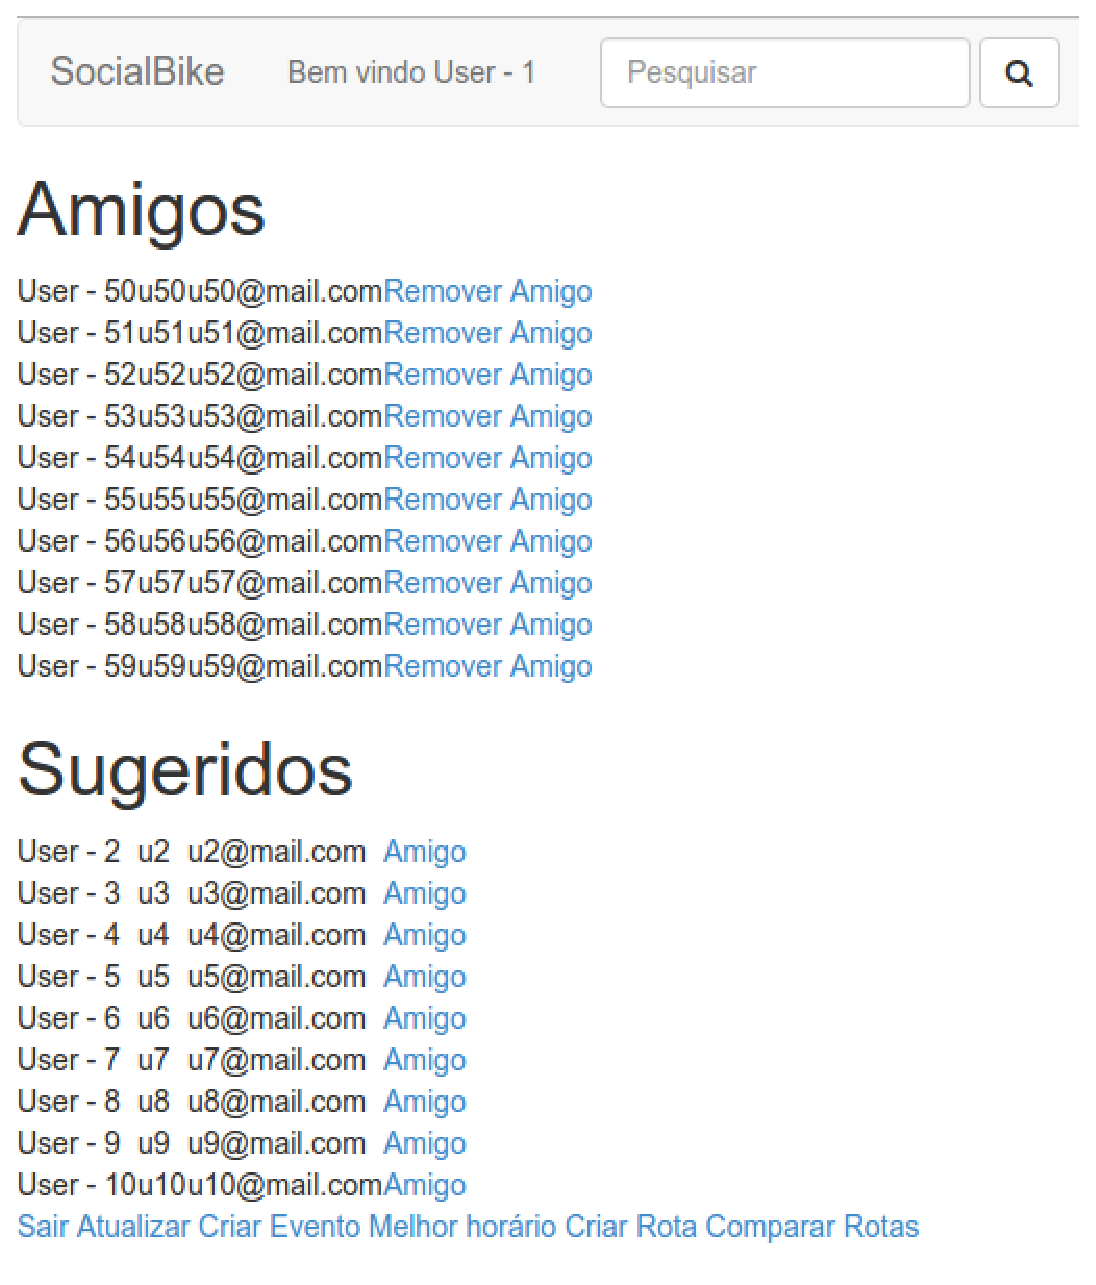
\includegraphics[scale=0.45]{figuras/resultados/home.eps}
	\caption[Tela principal]{Tela principal}
	\label{home}
\end{figure}

A Figura \ref{pesquisa} mostra os resultados retornados quando um usuário faz uma pesquisa. Ao se realizar uma pesquisa, é apresentado o botão ``Continuar'', para que o usuário continue retornando mais resultados da pesquisa realizada. Nesse caso a tabela com os resultados é incrementada.

\begin{figure}[!h]
	\centering
	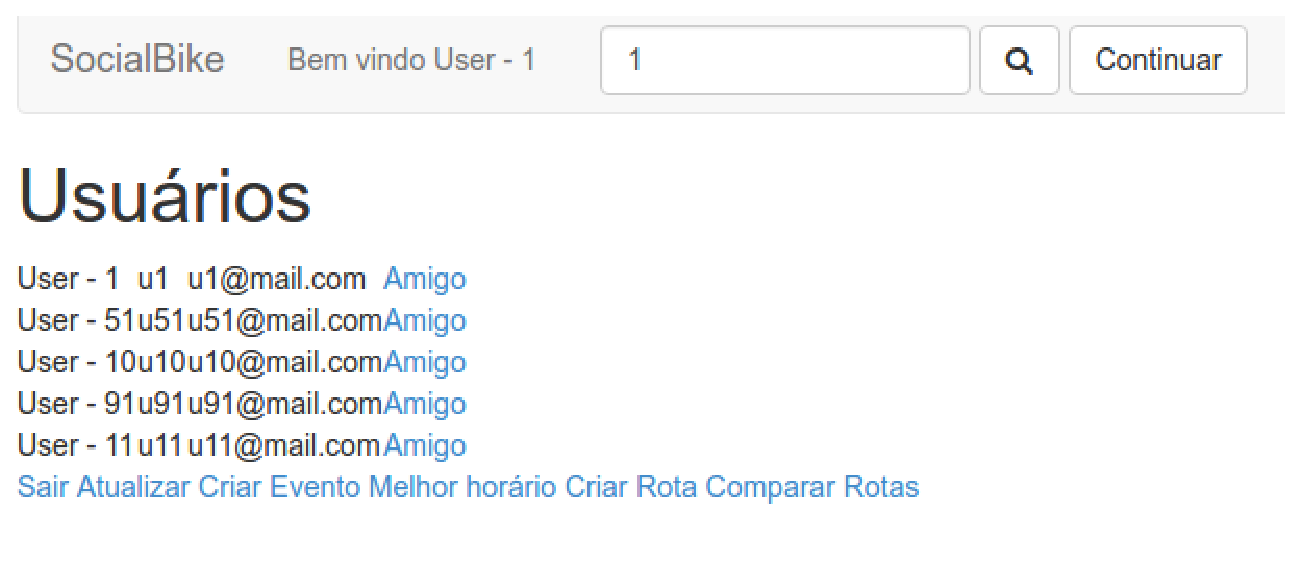
\includegraphics[scale=0.45]{figuras/resultados/pesquisa.eps}
	\caption[Resultados da pesquisa]{Resultados da pesquisa}
	\label{pesquisa}
\end{figure}

Na sequência, as Figuras \ref{criar_evento} e \ref{evento} mostram, respectivamente, as telas para criação de eventos e a visualização desses eventos, com a possibilidade de convidar usuários.

\newpage
\begin{figure}[!h]
	\centering
	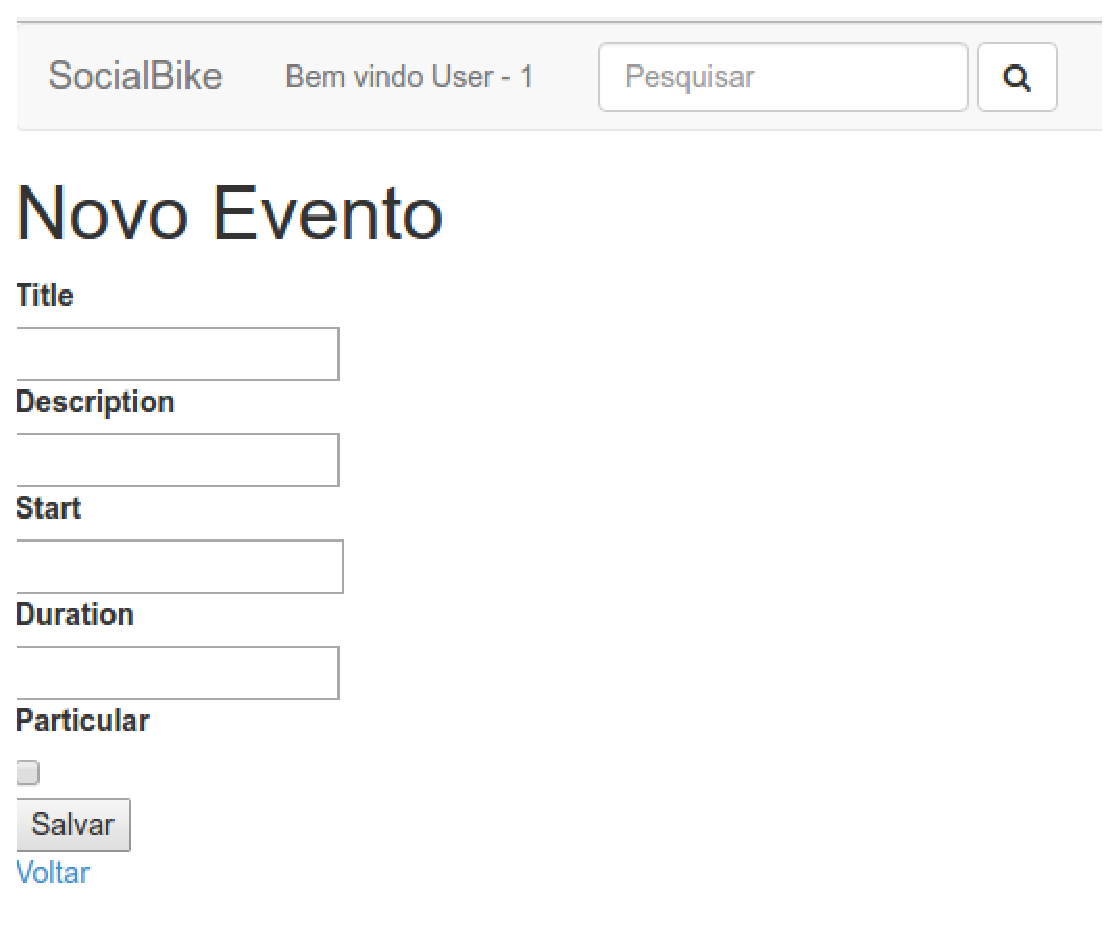
\includegraphics[scale=0.45]{figuras/resultados/criar_evento.eps}
	\caption[Criar Evento]{Criar Evento}
	\label{criar_evento}
\end{figure}

\begin{figure}[!h]
	\centering
	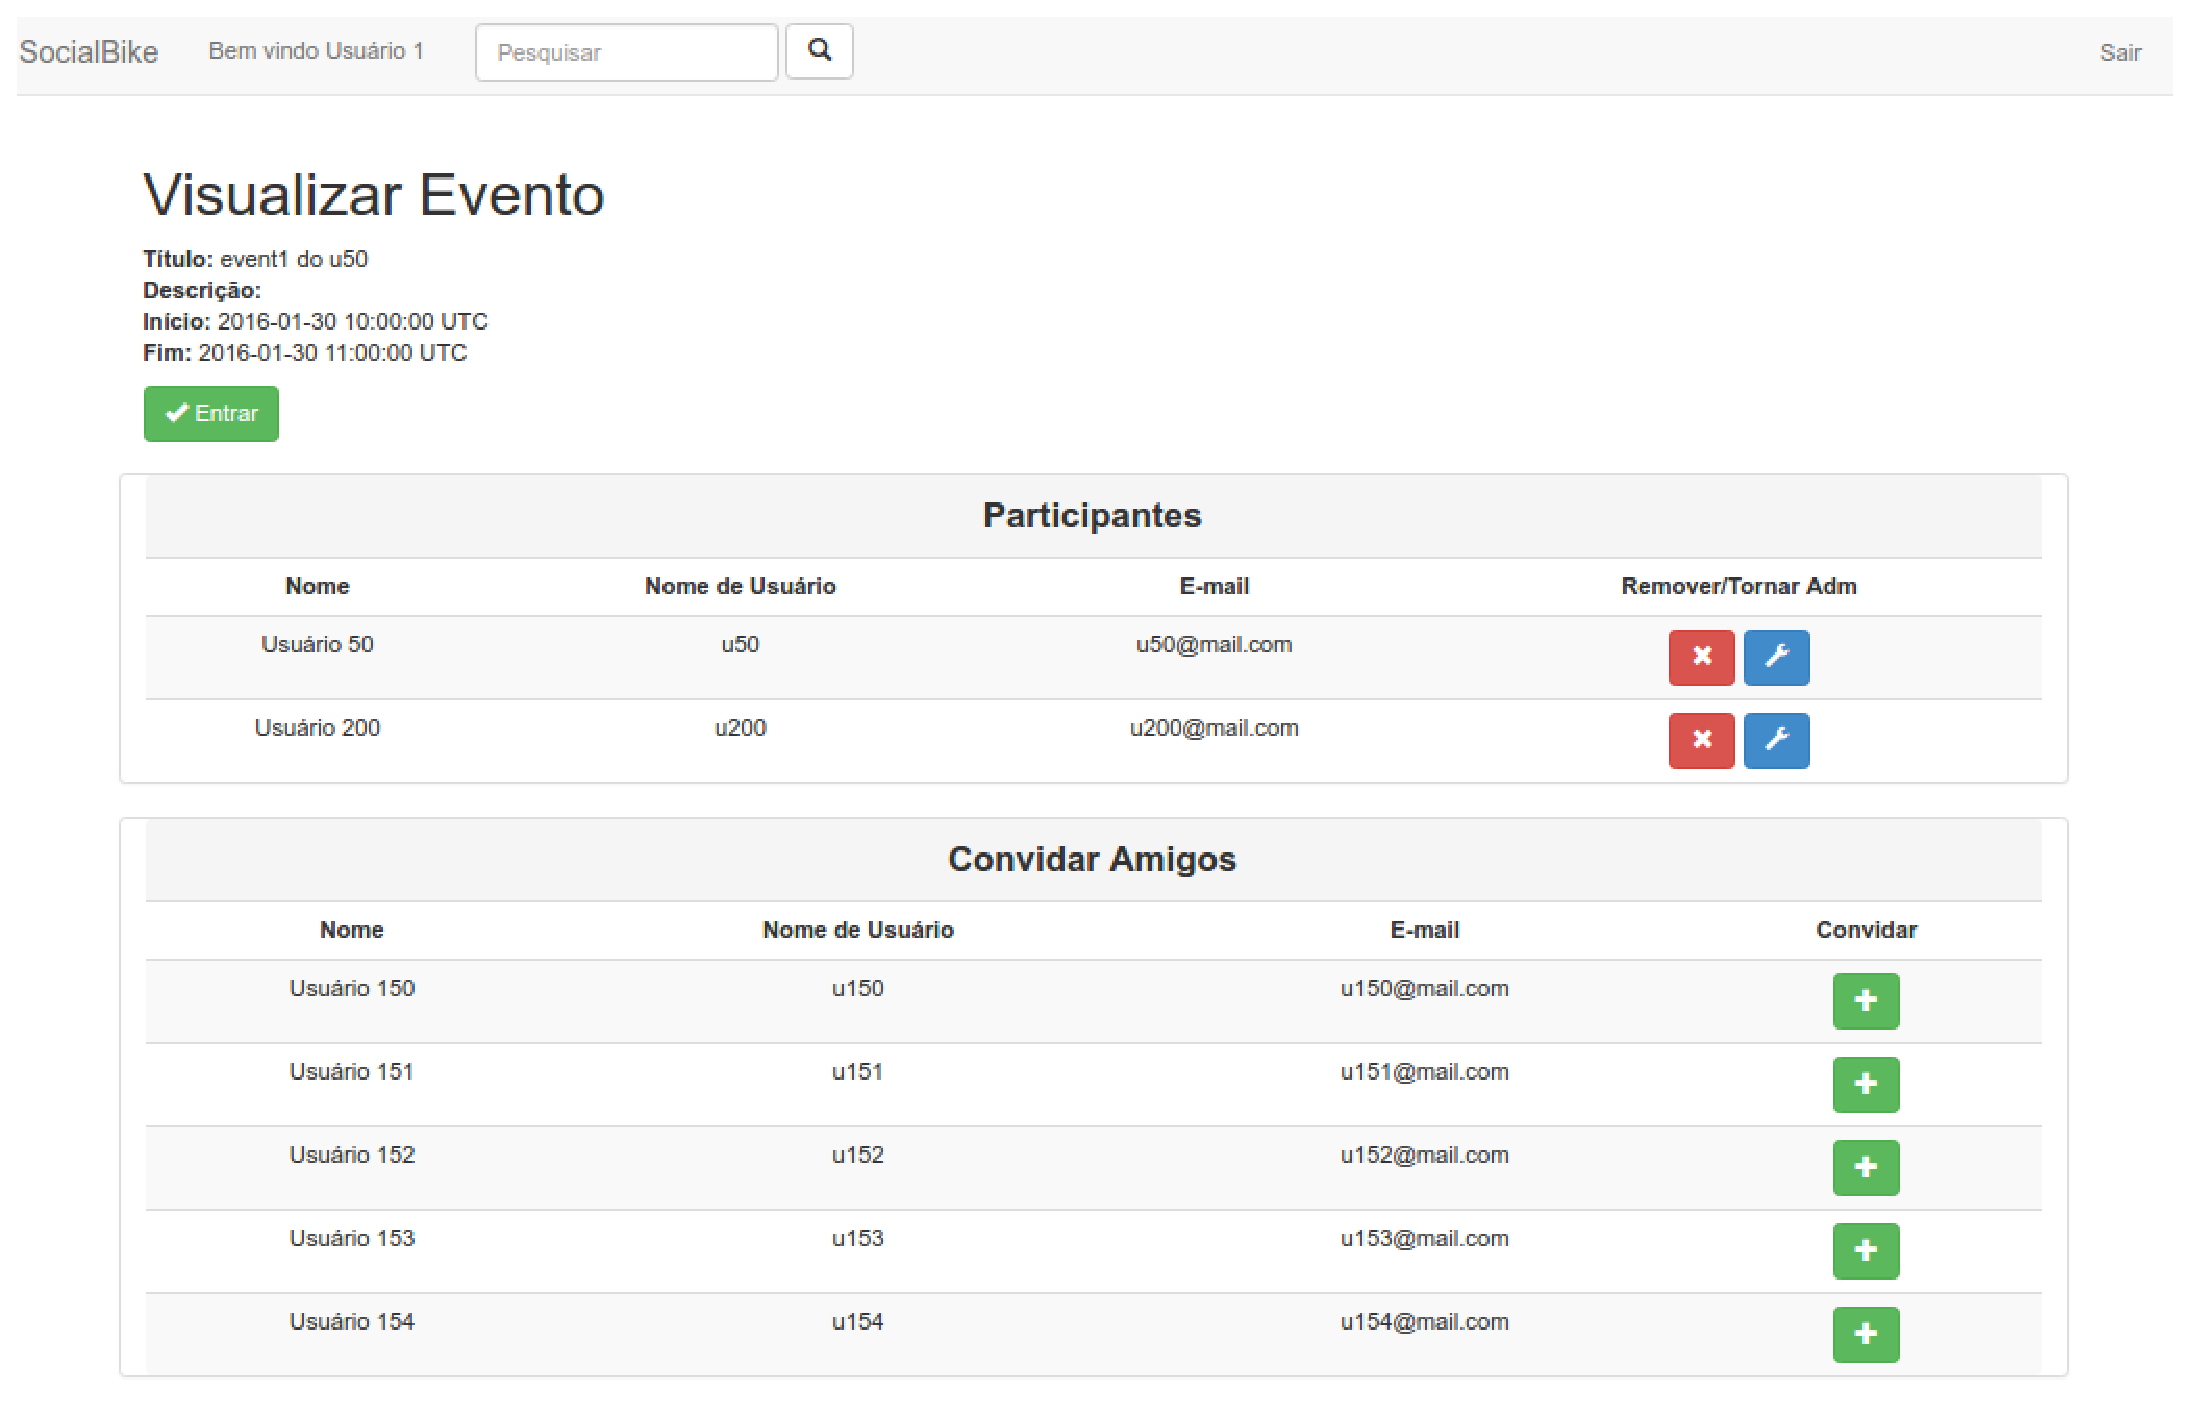
\includegraphics[scale=0.45]{figuras/resultados/evento.eps}
	\caption[Visualizar Evento]{Visualizar Evento}
	\label{evento}
\end{figure}

A tela apresentada na Figura \ref{compatibilidade_horarios} é usada para verificar a compatibilidade de horários para marcação de um evento em um determinado período de tempo. Têm-se a lista de amigos do usuário logado para que este possa adicioná-los juntamente com seus pesos para realizar a verificação. Outros atributos que devem ser passados são os já mencionados antes, os quais são necessários para a execução do algoritmo.

\newpage
\begin{figure}[!h]
	\centering
	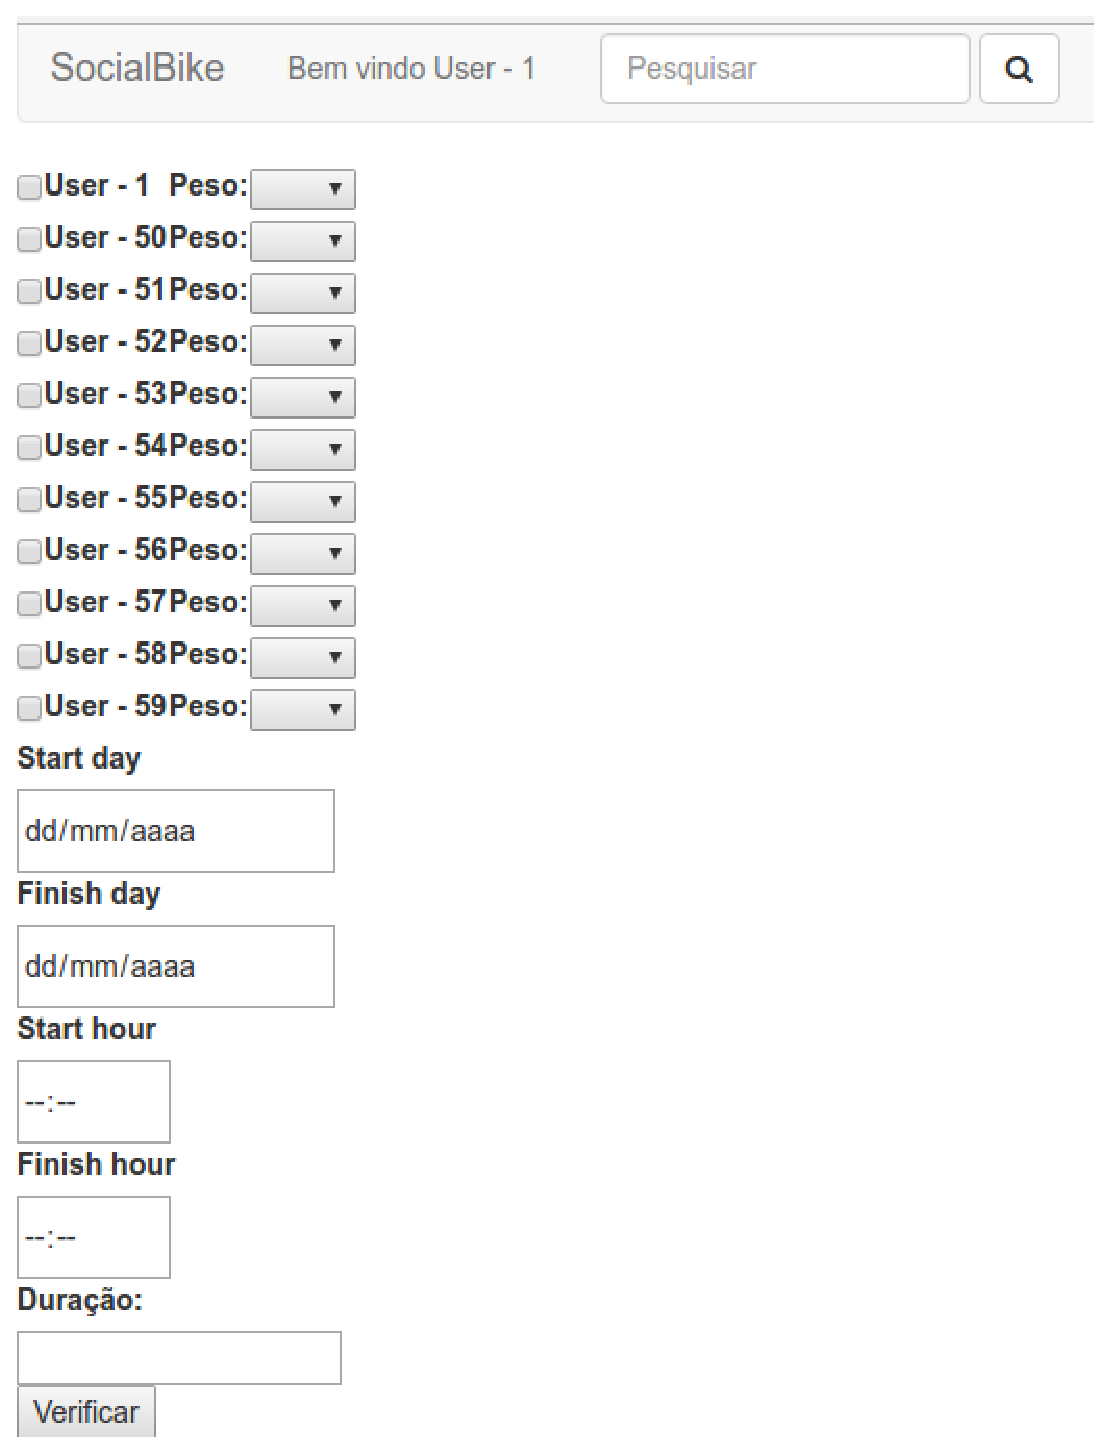
\includegraphics[scale=0.45]{figuras/resultados/compatibilidade_horarios.eps}
	\caption[Verificar compatibilidade de horários]{Verificar compatibilidade de horários}
	\label{compatibilidade_horarios}
\end{figure}

As Figuras \ref{cadastrar_rota} e \ref{ver_rota} mostram, respectivamente, as telas para criação e visualização de rotas.

\newpage
\begin{figure}[!h]
	\centering
	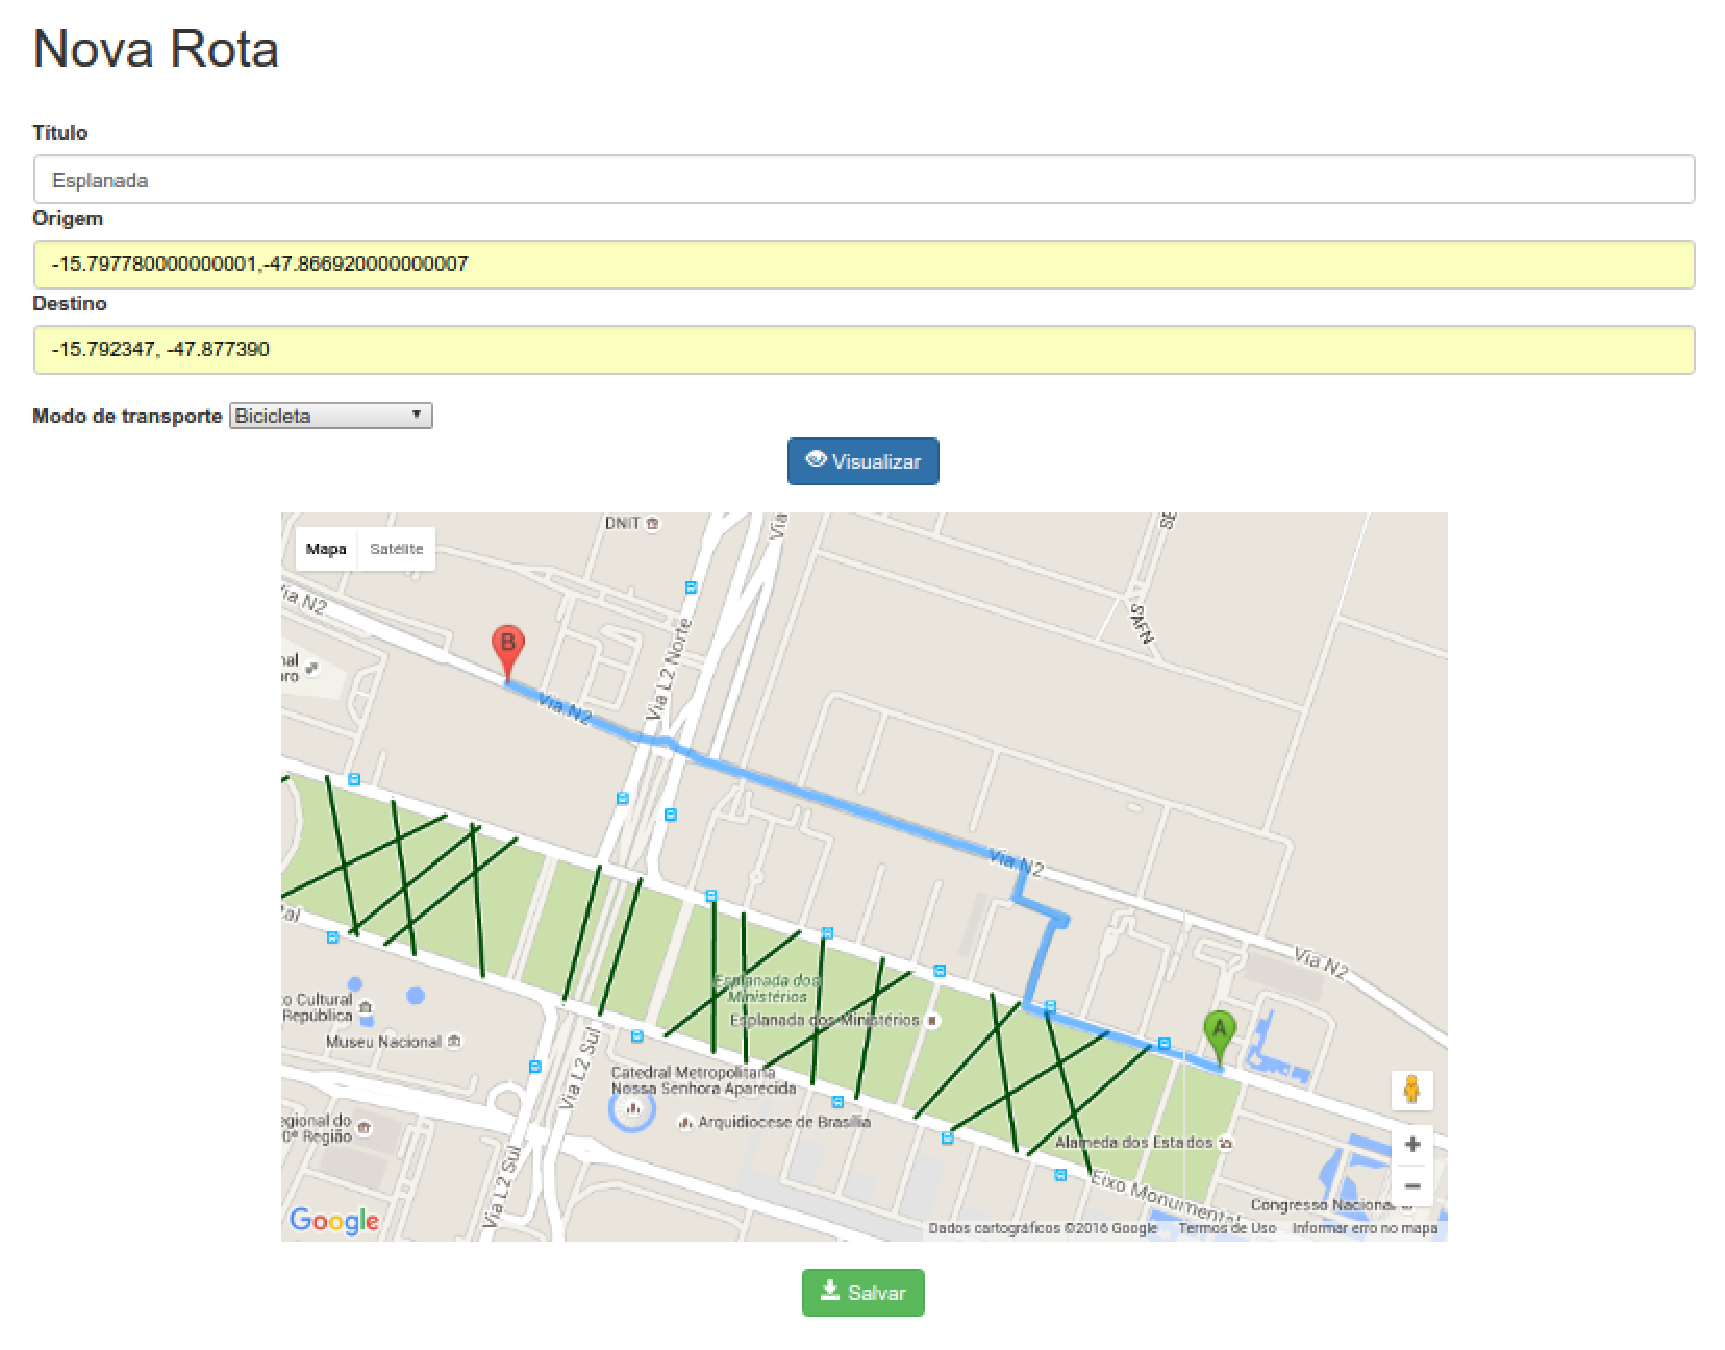
\includegraphics[scale=0.45]{figuras/resultados/cadastrar_rota.eps}
	\caption[Cadastrar Rota]{Cadastrar Rota}
	\label{cadastrar_rota}
\end{figure}

\begin{figure}[!h]
	\centering
	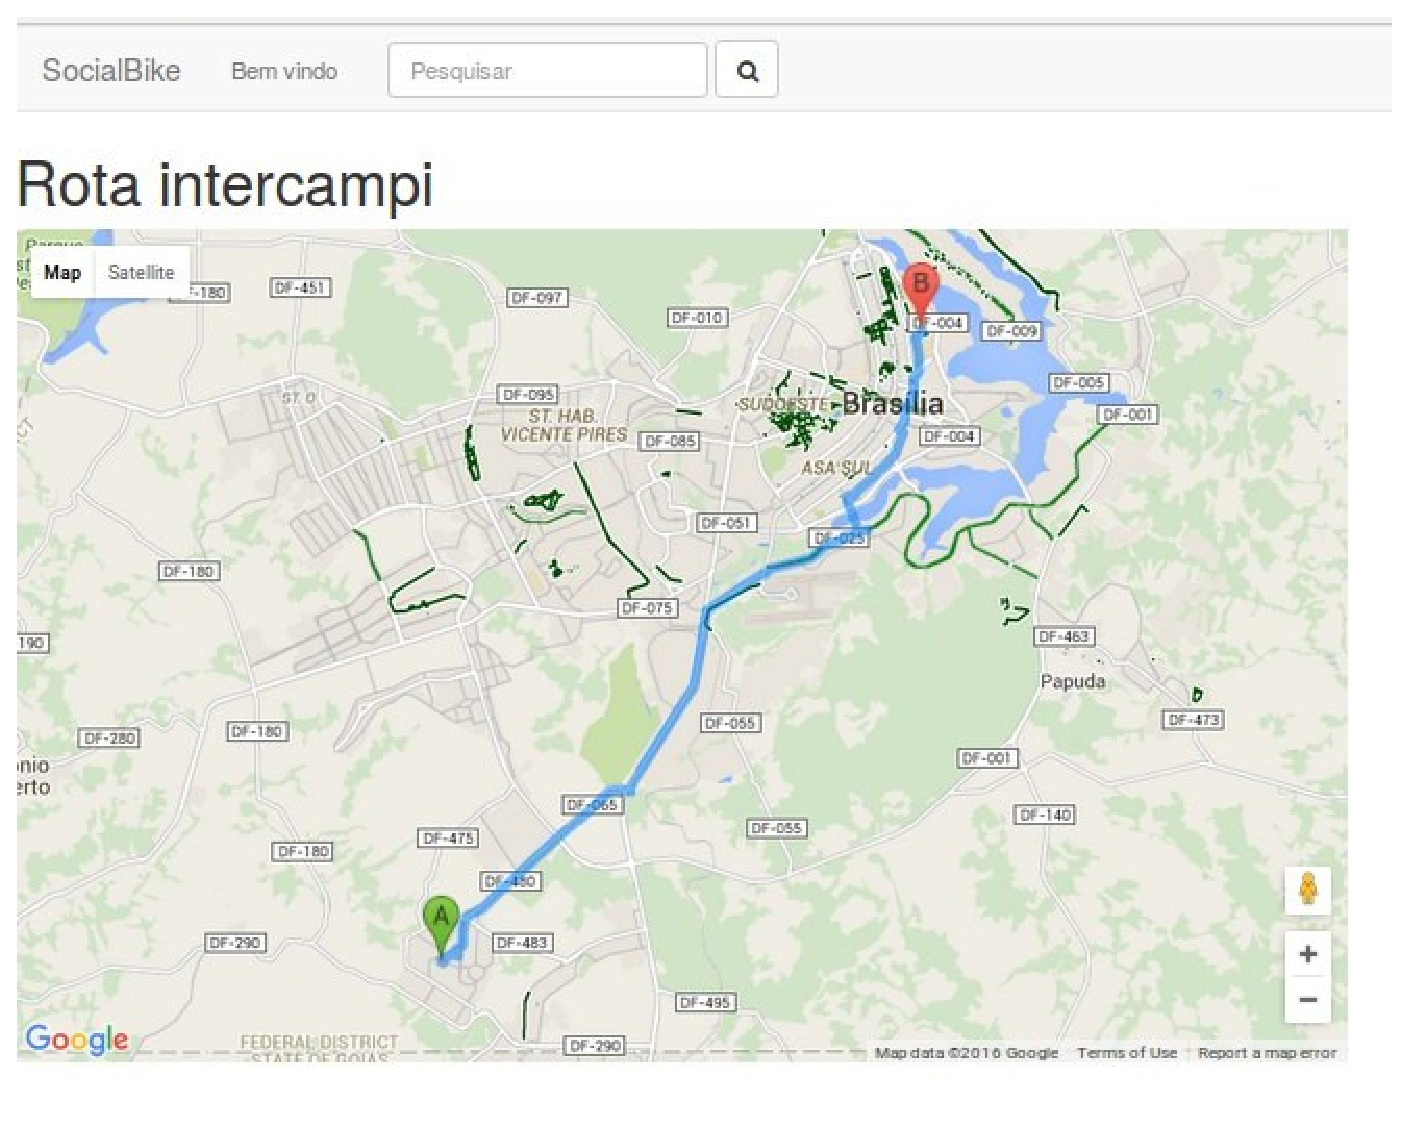
\includegraphics[scale=0.45]{figuras/resultados/ver_rota.eps}
	\caption[Visualizar Rota]{Visualizar Rota}
	\label{ver_rota}
\end{figure}

Por fim, têm-se as Figuras \ref{comparar_rotas} e \ref{resultado_comparacao}. Nessas imagens, pode-se ver um formulário para realizar a comparação entre duas rotas e o resultado dessa comparação, em que se percebe que as rotas são compatíveis e qual a nova distância total para a rota principal, que será alterada para atender a rota secundária.

\begin{figure}[!h]
	\centering
	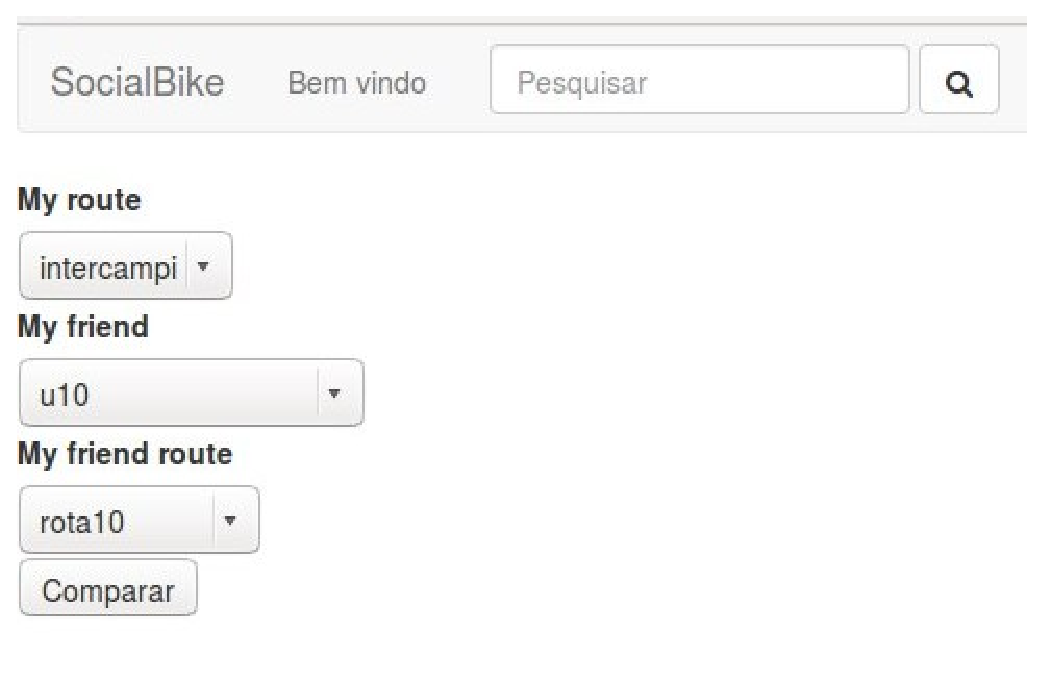
\includegraphics[scale=0.45]{figuras/resultados/comparar_rotas.eps}
	\caption[Comparar rotas]{Comparar rotas}
	\label{comparar_rotas}
\end{figure}

\begin{figure}[!h]
	\centering
	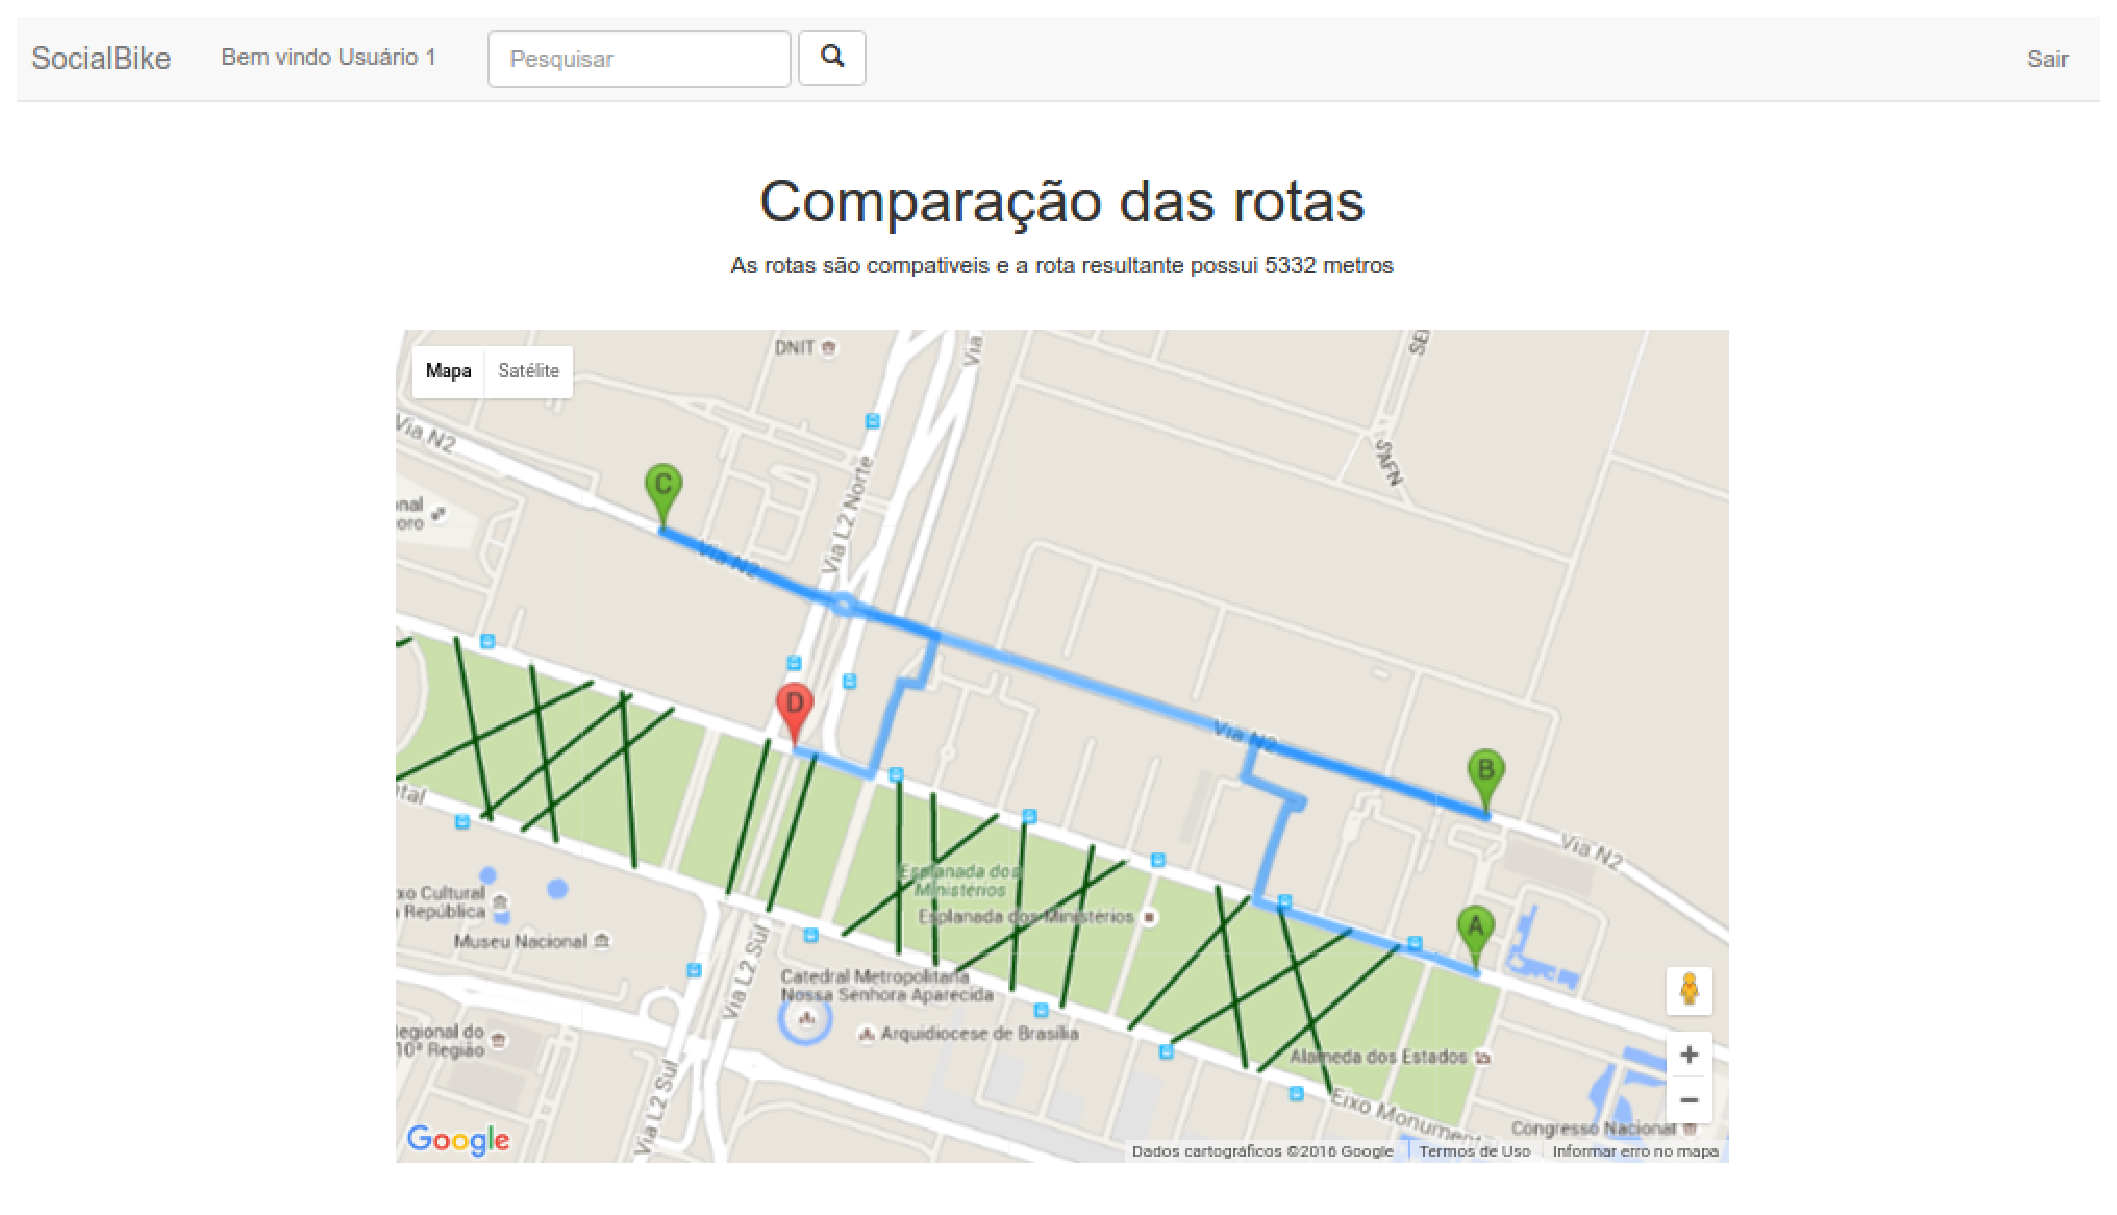
\includegraphics[scale=0.45]{figuras/resultados/resultado_comparacao.eps}
	\caption[Resultado da comparação]{Resultado da comparação}
	\label{resultado_comparacao}
\end{figure}

O código da SocialBike pode ser acessado através do endereço \url{https://github.com/TCC-SocialNetwork/social_bike}.

\section{Resumo do Capítulo}
Este capítulo foi responsável por apresentar os principais resultados obtidos ao longo do processo de desenvolvimento, tanto do SocialFramewok quanto da rede social SocialBike.

Foram apresentados alguns relatórios contendo os resultados. Um dos relatórios apresentados foi o relatório de testes. Nesse, constam a cobertura de código. Adicionalmente, foram apresentados os principais relatórios de desempenho, os quais mostram como os algoritmos se comportaram em complexidade e uso de memória. Por fim, têm-se os relatórios de qualidades, nos quais constam os resultados obtidos - utilizando o Code Climate - visando aferir as principais medidas de qualidade de código.

Além disso, foram apresentadas a rede social SocialBike e suas funcionalidades, as quais foram todas desenvolvidas a partir dos recursos do SocialFramework para uma melhor análise de uso do mesmo.
